\documentclass[aps,floatfix,prx,superscriptaddress,reprint,showpacs,10pt,preprintnumbers,longbibliography]{revtex4-2}

\usepackage[utf8]{inputenc}
\usepackage[pdftex]{graphicx}
\usepackage{float}
\usepackage{amssymb}
\usepackage{amsmath}  
\usepackage{amsfonts}
\usepackage{amsthm}
\usepackage{dsfont}
\usepackage{array}
\usepackage{bm}
\usepackage{mathrsfs}
\usepackage{pifont}
\usepackage{multirow}
\usepackage{upgreek}
\usepackage[dvipsnames]{xcolor}
\usepackage[pdftex,
            pdftitle={Materials Science Working Group - White Paper},
            pdfauthor={Authors},
            bookmarks,
            colorlinks,
            linkcolor=black,
            citecolor=mymagenta,
            menucolor=black,
            urlcolor=myblue,
            plainpages=false,
            pdfpagelabels,
            hypertexnames=false]{hyperref}
\usepackage{verbatim}
\usepackage{slashed}
\usepackage{bm}
\usepackage{braket}
\usepackage{booktabs}
\usepackage{multirow}
\usepackage{physics}
\usepackage{bm}
\usepackage{bbm}
\usepackage{tabularx}
\usepackage{makecell}
\usepackage{longtable}
\usepackage{textcomp}
\newcommand{\ce}[1]{$\mathrm{#1}$}
\usepackage[acronym,symbols,nogroupskip,nomain,nonumberlist,nopostdot,toc]{glossaries}
\definecolor{mymagenta}{RGB}{200, 0, 100}
\definecolor{myblue}{RGB}{45, 48, 146}



\graphicspath{{figures/}}


\newacronym{hep}{HEP}{High-Energy Physics}
\newacronym{qc}{QC}{Quantum Computing}
\newacronym{lgt}{LGT}{Lattice Gauge Theory}
\newacronym{qed}{QED}{Quantum Electrodynamics}
\newacronym{qcd}{QCD}{Quantum Chromodynamics}
\newacronym{tn}{TN}{Tensor Network}
\newacronym{qtn}{QTN}{Quantum Tensor Network}
\newacronym{vqe}{VQE}{Variational Quantum Eigensolver}
\newacronym{vqd}{VQD}{Variational Quantum Deflation}
\newacronym{ssvqe}{SSVQE}{Subspace-search Variational Quantum Eigensolver}
\newacronym{pf}{PF}{Product Formulas}
\newacronym{vte}{VTE}{Variational Time Evolution}
\newacronym{eom}{EOM}{Equation of Motion}
\newacronym{1p1D}{(1+1)D}{(1+1)-Dimensional}
\newacronym{2p1D}{(2+1)D}{(2+1)-Dimensional}
\newacronym{3p1D}{(3+1)D}{(3+1)-Dimensional}
\newacronym{cnot}{CNOT}{Controlled NOT gate}
\newacronym{mps}{MPS}{Matrix Product States}
\newacronym{zne}{ZNE}{Zero-Noise Extrapolation}
\newacronym{pec}{PEC}{probabilistic error cancellation}
\newacronym{qgan}{QGAN}{Quantum Generative Adversarial Network}
\newacronym{aqgan}{QGAN}{Anomaly Quantum Generative Adversarial Network}
\newacronym{qubo}{QUBO}{Quantum Unconstrained Binary Optimization}
\newacronym{hhl}{HHL}{Harrow-Hassidim-Lloyd}
\newacronym{qnn}{QNN}{Quantum Neural Network}
\newacronym{qaoa}{QAOA}{Quantum Approximate Optimization Algorithm}
\newacronym{qsvm}{QSVM}{Quantum-enhanced Support Vector Machine}
\newacronym{mcmc}{MCMC}{Markov Chain Monte Carlo}
\newacronym{bsm}{BSM}{Beyond the Standard Model}
\newacronym{sm}{SM}{Standard Model}
\newacronym{ks}{K-S}{Kogut-Susskind}
\newacronym{qkmeans}{QKMEANS}{Quantum k-means}
\newacronym{tda}{TDA}{Topological Data Analysis}
\newacronym{rl}{RL}{Reinforcement Learning}
\newacronym{qrl}{QRL}{Quantum Reinforcement Learning}
\newacronym{gnn}{GNN}{Graph Neural Network}
\newacronym{qgnn}{QGNN}{quantum-classical hybrid Graph Neural Network}
\newacronym{gpu}{GPU}{Graphics Processing Unit}
\newacronym{qml}{QML}{Quantum Machine Learning}
\newacronym{gqml}{GQML}{Geometrical Quantum Machine Learning}
\newacronym{vqa}{VQA}{Variational Quantum Algorithm}
\newacronym{qae}{QAE}{Quantum AutoEncoder}
\newacronym{csvc}{CSVC}{Classic Support Vector Classifier}
\newacronym{qsvc}{QSVC}{Quantum Support Vector Classifier}
\newacronym{nisq}{NISQ}{Noisy Intermediate-Scale Quantum}
\newacronym{vbs}{VBS}{Vector Boson Scattering}
\newacronym{ctf}{CTF}{Combinatorial Track Finder}
\newacronym{irc}{IRC}{Infrared and Collinear}
\newacronym{pdf}{PDF}{Parton Distribution Function}
\newacronym{eft}{EFT}{Effective Field Theory}
\newacronym{pdfs}{PDFs}{Parton Distribution Functions}
\newacronym{efts}{EFTs}{Effective Field Theories}
\newacronym{pqc}{PQC}{Parameterized Quantum Circuit}
\newacronym{varQTE}{varQTE}{variational Quantum Time Evolution}
\newacronym{varQITE}{varQITE}{variational Quantum Imaginary Time Evolution}
\newacronym{qcnn}{QCNN}{Quantum Convolutional Neural Network}
\newacronym{qcbm}{QCBM}{Quantum Circuit Born Machine}
\newacronym{povm}{POVM}{Positive Operator Valued Measure}
\newacronym{msw}{MSW}{Mikheyev-Smirnov-Wolfenstein}
\newacronym{cms}{CMS}{Compact Muon Solenoid}
\newacronym{qbm}{QBM}{Quantum Boltzmann Machine}


\makeglossaries


\newcommand{\oper}[1]{\hat{#1}} 
\newcommand{\N}{{\mathbb{N}}}
\newcommand{\Z}{{\mathbb{Z}}}
\newcommand{\R}{{\mathbb{R}}}
\newcommand{\C}{{\mathbb{C}}}
\newcommand{\CP}{{\mathbb{C}P}}
\newcommand{\1}{1\!\!1}
\newcommand{\0}{0\hspace{-1.65mm}0}
\newcommand{\p}{\partial}
\newcommand{\ontopof}[2]{\genfrac{}{}{0pt}{}{#1}{#2}}


\begin{document}


\newpage

\title{Quantum-centric Supercomputing for Materials Science:\\ \vspace{0.2cm}
A Perspective on Challenges and Future Directions \vspace{1.2cm}}

\author{Yuri Alexeev}
\affiliation{Argonne National Laboratory, Lemont, IL 60439, USA}

\author{Maximilian Amsler}
\affiliation{Corporate Sector Research and Advance Engineering, Robert Bosch GmbH, Robert-Bosch-Campus 1, D-71272 Renningen, Germany}

\author{Marco Antonio Barroca}
\affiliation{IBM Research, Rio de Janeiro, 20031-170, RJ, Brazil}
\affiliation{Centro Brasileiro de Pesquisas F\'isicas, Rio de Janeiro, 22290-180, RJ, Brazil}

\author{Sanzio Bassini}
\affiliation{CINECA, Bologna, Italy}

\author{Torey Battelle}
\affiliation{Arizona State University, USA}

\author{Daan Camps}
\affiliation{National Energy Research Scientific Computing Center, Lawrence Berkeley National Laboratory Berkeley, CA, USA}

\author{David Casanova}
\affiliation{Donostia International Physics Center (DIPC), 20018 Donostia-San Sebasti\'an, Euskadi, Spain}
\affiliation{Ikerbasque, Basque Foundation for Science, 48009 Bilbao, Spain}

\author{Young jai Choi}
\affiliation{Department of Physics, Yonsei University, Seoul 03722, Korea}

\author{Frederic T. Chong}
\affiliation{University of Chicago, Chicago, Illinois, USA}

\author{Charles Chung}
\affiliation{IBM Quantum, IBM T.J. Watson Research Center, Yorktown Heights, NY 10598, USA}

\author{Chris Codella}
\affiliation{IBM Quantum, IBM T.J. Watson Research Center, Yorktown Heights, NY 10598, USA}

\author{Antonio D. C\'orcoles}
\affiliation{IBM Quantum, IBM T.J. Watson Research Center, Yorktown Heights, NY 10598, USA}

\author{James Cruise}
\affiliation{Cambridge Consultants part of Capgemini Invent, Cambridge, UK }

\author{Alberto Di Meglio}
\affiliation{European Organization for Nuclear Research (CERN), Geneva 1211, Switzerland}

\author{Ivan Duran}
\affiliation{IBM Quantum, IBM T.J. Watson Research Center, Yorktown Heights, NY 10598, USA}

\author{Thomas Eckl}
\affiliation{Corporate Sector Research and Advance Engineering, Robert Bosch GmbH, Robert-Bosch-Campus 1, D-71272 Renningen, Germany}

\author{Sophia Economou}
\affiliation{Virginia Tech, Blacksburg, VA 24061, USA}

\author{Stephan Eidenbenz}
\affiliation{Los Alamos National Laboratory, Los Alamos, NM 87545, USA}

\author{Bruce Elmegreen}
\affiliation{IBM Quantum, IBM T.J. Watson Research Center, Yorktown Heights, NY 10598, USA}

\author{Clyde Fare}
\affiliation{IBM Quantum, IBM T.J. Watson Research Center, Yorktown Heights, NY 10598, USA}

\author{Ismael Faro}
\affiliation{IBM Quantum, IBM T.J. Watson Research Center, Yorktown Heights, NY 10598, USA}

\author{Cristina Sanz Fernández}
\affiliation{IBM Quantum, IBM T.J. Watson Research Center, Yorktown Heights, NY 10598, USA}

\author{Rodrigo Neumann Barros Ferreira}
\affiliation{IBM Research, Rio de Janeiro, 20031-170, RJ, Brazil}

\author{Keisuke Fuji}
\affiliation{Osaka University, Osaka 560-8531, Japan}

\author{Bryce Fuller}
\affiliation{IBM Quantum, IBM T.J. Watson Research Center, Yorktown Heights, NY 10598, USA}

\author{Laura Gagliardi}
\affiliation{Department of Chemistry, Chicago Center for Theoretical Chemistry, University of Chicago, Chicago, Illinois, USA}
\affiliation{Argonne National Laboratory, Lemont, IL 60439, USA}

\author{Giulia Galli}
\affiliation{University of Chicago, Chicago, Illinois, USA}
\affiliation{Argonne National Laboratory, Lemont, IL 60439, USA}

\author{Jennifer R. Glick}
\affiliation{IBM Quantum, IBM T.J. Watson Research Center, Yorktown Heights, NY 10598, USA}

\author{Isacco Gobbi}
\affiliation{Fraunhofer ITWM, Kaiserslautern, Rheinland-Pfalz 67663, DE}

\author{Pranav Gokhale}
\affiliation{Infleqtion, Chicago, IL 60622, USA}

\author{Salvador de la Puente Gonzalez}
\affiliation{IBM Quantum, IBM T.J. Watson Research Center, Yorktown Heights, NY 10598, USA}

\author{Johannes Greiner}
\affiliation{IBM Quantum, IBM T.J. Watson Research Center, Yorktown Heights, NY 10598, USA}

\author{Bill Gropp}
\affiliation{University of Illinois Urbana-Champaign}

\author{Michele Grossi}
\affiliation{European Organization for Nuclear Research (CERN), Geneva 1211, Switzerland}

\author{Emmanuel Gull}
\affiliation{University of Michigan, Ann Arbor, Michigan 48109, USA}

\author{Burns Healy}
\affiliation{Dell Technologies, Research Office}

\author{Benchen Huang}
\affiliation{University of Chicago, Chicago, Illinois, USA}

\author{Travis S.~Humble}
\affiliation{Oak Ridge National Laboratory, One Bethel Valley Road, Oak Ridge, 37831, Tennessee, USA}

\author{Nobuyasu Ito}
\affiliation{RIKEN Center for Computational Science (R-CCS), Kobe, Hyogo 650-0047, Japan}

\author{Artur F. Izmaylov}
\affiliation{Chemical Physics Theory Group, Department of Chemistry, University of Toronto, Toronto, Ontario M5S 3H6, Canada}
\affiliation{Department of Physical and Environmental Sciences, University of Toronto Scarborough, Toronto, Ontario M1C 1A4, Canada}

\author{Ali Javadi-Abhari}
\affiliation{IBM Quantum, IBM T.J. Watson Research Center, Yorktown Heights, NY 10598, USA}

\author{Douglas Jennewein}
\affiliation{Arizona State University, USA}

\author{Shantenu Jha}
\affiliation{Brookhaven National Laboratory, Upton, NY, USA}
\affiliation{Rutgers University, New Brunswick, NJ, USA}

\author{Liang Jiang}
\affiliation{University of Chicago, Chicago, Illinois, USA}

\author{Barbara Jones}
\affiliation{IBM Research, Almaden Lab, San Jose, CA 95120, USA}

\author{Wibe Albert de Jong}
\affiliation{Applied Mathematics and Computational Research Division, Lawrence Berkeley National Laboratory, Berkeley, California 94720, USA}

\author{Petar Jurcevic}
\affiliation{IBM Quantum, IBM T.J. Watson Research Center, Yorktown Heights, NY 10598, USA}

\author{William Kirby}
\affiliation{IBM Quantum, IBM Research Cambridge, Cambridge, MA 02142, USA}

\author{Stefan Kister}
\affiliation{IBM Quantum, IBM T.J. Watson Research Center, Yorktown Heights, NY 10598, USA}

\author{Masahiro Kitagawa}
\affiliation{Osaka University, Osaka 560-8531, Japan}

\author{Joel Klassen}
\affiliation{Phasecraft Ltd., London, UK}

\author{Katherine Klymko}
\affiliation{National Energy Research Scientific Computing Center Lawrence Berkeley National Laboratory Berkeley, CA, USA}

\author{Kwangwon Koh}
\affiliation{Electronics and Telecommunications Research Institute (ETRI), Daejeon, Republic of Korea}

\author{Masaaki Kondo}
\affiliation{Keio University, Yokohama, Kanagawa 223-8522, Japan}
\affiliation{RIKEN Center for Computational Science (R-CCS), Kobe, Hyogo 650-0047, Japan}

\author{Do\~ga Murat K\"urk\c{c}\"uo\~glu}
\affiliation{Fermi National Accelerator Laboratory, Batavia, IL 60510, USA}
\affiliation{Superconducting Quantum Materials and Systems Center (SQMS),
Fermi National Accelerator Laboratory, Batavia, IL 60510, USA}

\author{Krzysztof Kurowski}
\affiliation{Poznań Supercomputing and Networking Center, IBCH PAS Poznań, Poland}

\author{Teodoro Laino}
\affiliation{IBM Research Europe, S\"aumerstrasse 4, 8803 R\"uschlikon, Switzerland}

\author{Ryan Landfield}
\affiliation{Oak Ridge National Laboratory, One Bethel Valley Road, Oak Ridge, 37831, Tennessee, USA}

\author{Matt Leininger}
\affiliation{Lawrence Livermore National Laboratory, Livermore, California 94550, USA}

\author{Vicente Leyton-Ortega}
\affiliation{Oak Ridge National Laboratory, One Bethel Valley Road, Oak Ridge, 37831, Tennessee, USA}

\author{Ang Li}
\affiliation{Pacific Northwest National Laboratory, Richland, Washington 99354, USA}
\affiliation{University of Washington, Seattle, Washington 98195, USA}

\author{Meifeng Lin}
\affiliation{Brookhaven National Laboratory, Upton, NY, USA}

\author{Junyu Liu}
\affiliation{University of Chicago, Chicago, Illinois, USA}


\author{Nicolas Lorente}
\affiliation{Centro de Fisica de Materiales (CSIC-EHU), 20018 Donostia-San Sebasti\'an, Euskadi, Spain}
\affiliation{Donostia International Physics Center (DIPC), 20018 Donostia-San Sebasti\'an, Euskadi, Spain}

\author{Andre Luckow}
\affiliation{BMW Group, Munich, Germany}

\author{Simon Martiel}
\affiliation{IBM Quantum, IBM T.J. Watson Research Center, Yorktown Heights, NY 10598, USA}

\author{Francisco Martin-Fernandez}
\affiliation{IBM Quantum, IBM T.J. Watson Research Center, Yorktown Heights, NY 10598, USA}

\author{Margaret Martonosi}
\affiliation{Princeton University, Princeton, New Jersey, USA}

\author{Claire Marvinney}
\affiliation{Oak Ridge National Laboratory, One Bethel Valley Road, Oak Ridge, 37831, Tennessee, USA}

\author{Arcesio Castaneda Medina}
\affiliation{Fraunhofer ITWM, Kaiserslautern, Rheinland-Pfalz 67663, DE}

\author{Dirk Merten}
\affiliation{Fraunhofer ITWM, Kaiserslautern, Rheinland-Pfalz 67663, DE}

\author{Antonio Mezzacapo}
\email{mezzacapo@ibm.com}
\affiliation{IBM Quantum, IBM T.J. Watson Research Center, Yorktown Heights, NY 10598, USA}


\author{Kristel Michielsen}
\affiliation{J\"ulich Supercomputing Centre, Institute for Advanced Simulation, Forschungszentrum J\"ulich, 52425 J\"ulich, Germany}

\author{Abhishek Mitra}
\affiliation{Department of Chemistry, Chicago Center for Theoretical Chemistry, University of Chicago, Chicago, Illinois, USA}

\author{Tushar Mittal}
\affiliation{IBM Quantum, IBM T.J. Watson Research Center, Yorktown Heights, NY 10598, USA}

\author{Kyungsun Moon}
\affiliation{Department of Physics, Yonsei University, Seoul 03722, Korea}

\author{Joel Moore}
\affiliation{University of California, Berkeley, California 94720, USA}
\affiliation{National Energy Research Scientific Computing Center, Lawrence Berkeley National Laboratory, Berkeley, CA, USA}

\author{Mario Motta}
\affiliation{IBM Quantum, IBM T.J. Watson Research Center, Yorktown Heights, NY 10598, USA}

\author{Young-Hye Na}
\affiliation{IBM Quantum, IBM T.J. Watson Research Center, Yorktown Heights, NY 10598, USA}

\author{Yunseong Nam}
\affiliation{IBM Quantum, IBM T.J. Watson Research Center, Yorktown Heights, NY 10598, USA}

\author{Prineha Narang}
\affiliation{Brookhaven National Laboratory, Upton, NY, USA}
\affiliation{University of California Los Angeles, Los Angeles, California 90095, USA}

\author{Yu-ya Ohnishi}
\affiliation{JSR Corporation, 3-103-9, Tonomachi, Kawasaki-ku, Kawasaki, Kanagawa, 210-0821, Japan}

\author{Daniele Ottaviani}
\affiliation{CINECA}

\author{Matthew Otten}
\affiliation{Department of Physics, University of Wisconsin - Madison, Madison, WI 53706, USA}

\author{Scott Pakin}
\affiliation{Los Alamos National Laboratory, Los Alamos, NM 87545, USA}

\author{Vincent R. Pascuzzi}
\affiliation{IBM Quantum, IBM T.J. Watson Research Center, Yorktown Heights, NY 10598, USA}

\author{Ed Penault}
\affiliation{IBM Quantum, IBM T.J. Watson Research Center, Yorktown Heights, NY 10598, USA}

\author{Tomasz Piontek}
\affiliation{Poznań Supercomputing and Networking Center, IBCH PAS Poznań, Poland}

\author{Jed Pitera}
\affiliation{IBM Research, IBM Almaden Research Center, San Jose, CA 94028, USA}

\author{Patrick Rall}
\affiliation{IBM Quantum, IBM Research Cambridge, Cambridge, MA 02142, USA}

\author{Gokul Subramanian Ravi}
\affiliation{University of Michigan, Ann Arbor, Michigan 48109, USA}

\author{Niall Robertson}
\affiliation{IBM Quantum, IBM Research Europe - Dublin, IBM Technology Campus, Dublin 15, Ireland}

\author{Matteo Rossi}
\affiliation{Algorithmiq Ltd, Kanavakatu 3 C, FI-00160 Helsinki, Finland}

\author{Piotr Rydlichowski}
\affiliation{Poznań Supercomputing and Networking Center, IBCH PAS Poznań, Poland}

\author{Hoon Ryu}
\affiliation{Korea Institute of Science and Technology Information, Daejeon 34141, Republic of Korea}

\author{Georgy Samsonidze}
\affiliation{Robert Bosch LLC, Research and Technology Center, Sunnyvale, CA 94085, USA}

\author{Mitsuhisa Sato}
\affiliation{RIKEN Center for Computational Science (R-CCS), Kobe, Hyogo 650-0047, Japan}

\author{Nishant Saurabh}
\affiliation{Department of Information and Computing Sciences, Utrecht University, NL}

\author{Vidushi Sharma}
\affiliation{IBM Quantum, IBM T.J. Watson Research Center, Yorktown Heights, NY 10598, USA}

\author{Kunal Sharma}
\affiliation{IBM Quantum, IBM T.J. Watson Research Center, Yorktown Heights, NY 10598, USA}

\author{Soyoung Shin}
\affiliation{IBM Quantum, Almaden Research Center, San Jose, California 95120, USA}

\author{George Slessman}
\affiliation{CR8DL, Inc., USA} 

\author{Mathias Steiner}
\affiliation{IBM Research, Rio de Janeiro, 20031-170, RJ, Brazil}

\author{Iskandar Sitdikov}
\affiliation{IBM Quantum, IBM T.J. Watson Research Center, Yorktown Heights, NY 10598, USA}

\author{In-Saeng Suh}
\affiliation{Oak Ridge National Laboratory, One Bethel Valley Road, Oak Ridge, 37831, Tennessee, USA}

\author{Eric Switzer}
\affiliation{Donostia International Physics Center (DIPC), 20018 Donostia-San Sebasti\'an, Euskadi, Spain}

\author{Wei Tang}
\affiliation{Princeton University, Princeton, New Jersey, USA}

\author{Joel Thompson}
\affiliation{Applied Mathematics, Boeing Research \& Technology, Huntsville, AL 35824}

\author{Synge Todo}
\affiliation{The University of Tokyo 7-3-1 Hongo, Bunkyo-ku, Tokyo, Japan}

\author{Minh Tran}
\affiliation{IBM Quantum, IBM Research Cambridge, Cambridge, MA 02142, USA}

\author{Dimitar Trenev}
\affiliation{ExxonMobil Technology and Engineering Company, Annandale, NJ 08801, USA}



\author{Christian Trott}
\affiliation{Sandia National Laboratories, Albuquerque, NM, USA}

\author{Huan-Hsin Tseng}
\affiliation{Brookhaven National Laboratory, Upton, NY, USA}

\author{Esin Tureci}
\affiliation{Princeton University, Princeton, New Jersey, USA}

\author{David García Valiñas}
\affiliation{IBM Quantum, IBM T.J. Watson Research Center, Yorktown Heights, NY 10598, USA}

\author{Sofia Vallecorsa}
\affiliation{European Organization for Nuclear Research (CERN), Geneva 1211, Switzerland}

\author{Christopher Wever}
\affiliation{Corporate Sector Research and Advanced Engineering, Robert Bosch GmbH, Robert-Bosch-Campus 1, D-71272 Renningen, Germany}

\author{Konrad Wojciechowski}
\affiliation{Poznań Supercomputing and Networking Center, IBCH PAS Poznań, Poland}

\author{Xiaodi Wu}
\affiliation{University of Maryland, College Park, USA}

\author{Shinjae Yoo}
\affiliation{Brookhaven National Laboratory, Upton, NY, USA}

\author{Nobuyuki Yoshioka}
\affiliation{The University of Tokyo 7-3-1 Hongo, Bunkyo-ku, Tokyo, Japan}

\author{Victor Wen-zhe Yu}
\affiliation{Argonne National Laboratory, Lemont, IL 60439, USA}

\author{Seiji Yunoki}
\affiliation{RIKEN Center for Computational Science (R-CCS), Kobe, Hyogo 650-0047, Japan}
\affiliation{RIKEN Center for Quantum Computing (RQC), Wako, Saitama 351-0198, Japan}

\author{Sergiy Zhuk}
\affiliation{IBM Quantum, IBM Research Europe - Dublin, IBM Technology Campus, Dublin 15, Ireland}

\author{Dmitry Zubarev}
\affiliation{IBM Quantum, IBM T.J. Watson Research Center, Yorktown Heights, NY 10598, USA}


\date{\today}

\begin{abstract}
Computational models are an essential tool for the design, characterization, and discovery of novel materials. Hard computational tasks in materials science stretch the limits of existing high-performance supercomputing centers, consuming much of their simulation, analysis, and data resources. Quantum computing, on the other hand, is an emerging technology with the potential to accelerate many of the computational tasks needed for materials science. In order to do that, the quantum technology must interact with conventional high-performance computing in several ways: approximate results validation, identification of hard problems, and synergies in quantum-centric supercomputing. 
In this paper, we provide a perspective on how quantum-centric supercomputing can help address critical computational problems in materials science, the challenges to face in order to solve representative use cases, and new suggested directions.
 
\end{abstract}


\maketitle

\section{Introduction}
\label{Introduction}

This article reports on scientific discussions and conclusions elaborated at a workshop on \gls{hep} held in November 2022 at CERN in Geneva.
This first event of the Quantum Computing for HEP (QC4HEP) Working Group gathered experts on \gls{hep} from different academic and research institutions and countries over four continents, who besides being world experts in theoretical and experimental aspects of \gls{hep}, also shared a common interest in \gls{qc} and its potential as a game changer in the field. 
The main goal of the workshop, and of this report-article, is to set a common roadmap for selected topics of interest to this community, in which we believe that \gls{qc} can have a significant impact in the near future. 
To this end, we have investigated classes of problems and corresponding quantum algorithms that can lead to potential quantum advantage with near-term, noisy, quantum devices, and - in particular - using IBM superconducting devices. We aim at delivering a set of physically relevant use cases that can become interesting %playground for the 
demonstrations in view of the $100 \otimes 100$ challenge announced by IBM~\cite{IBM_100by100}. 

For practical purposes, we have organized this article into two main domain areas: theoretical methods and algorithms for modelling \gls{hep} problems, and numerical methods for the interpretation and analysis of experimental results as well as detector simulation and event generation. 
We strongly believe that there are important connections between the two research domains, where many of the quantum algorithms designed for the solution of problems in one field can also be transferred to the other. 

We will therefore start with a short summary of the main \gls{hep} domains in theoretical modelling and experimental physics, for which we believe there is the potential for quantum computing to play a significant role in the near-term.  


\subsection{Quantum Computing for Theoretical Modelling in \gls{hep}}

Despite the great success of classical lattice field theory (e.g., for \gls{qed} and \gls{qcd} simulations~\cite{Durr2008,Alexandrou2020}), out-of-equilibrium and real-time dynamics (e.g., of particle collisions, thermalization phenomena or dynamics after a quench), remain out of reach for euclidean path-integral Monte Carlo simulations. 
Furthermore, properties of nuclear matter at high fermionic densities, as they arise in neutron stars or at the very early universe  for example, can not be accessed through these classical simulation techniques~\cite{Fukushima2011}. The same holds true for theories with topological terms, which are relevant, e.g. in \gls{qcd} for understanding the amount of CP-violation or, in the electroweak sector, the sphaleron rate in the early universe.  
These severe limitations are rooted in the notorious \emph{sign-problem}: the highly oscillatory behaviour of the path integrals arising in real-time phenomena, in systems with a high fermionic particle density or in the presence of topological terms imply an exponentially growing sampling run-time complexity with an increasing number of lattice sites~\cite{Troyer2005}.

An alternative approach to circumvent the sign problem might be to describe lattice fields theories in the equivalent Hamiltonian formalism, instead of the path integral description based on the Lagrangian formalism~\cite{Kogut1975,Kogut1979}. 
In the Hamiltonian approach, however, the total many-particle wave function which describes a general particle state on the whole lattice must be stored throughout the simulation. 
But since the total discretized Hilbert space $\mathcal{H}$ containing these general states corresponds to a tensor product of Hilbert spaces $\mathcal{H}_j$ on a single lattice site, the required memory to store a full wave function on the lattice scales exponentially with the number of lattice sites.

In recent years, novel tensor network-based methods have been introduced to alleviate these limitations by allowing for a more compact representation of general quantum states on the lattice~\cite{Silvi2014,Dalmonte2016,Banuls2019SimulatingLG,Banuls2019,Banuls2020TNreview}. The underlying mechanism which allows Hamiltonian simulations to be performed is that only a small subspace of the complete Hilbert space describes the low energy physics of quantum field theories and \gls{tn} methods identify and focus exactly on these physically relevant subspaces. Hence, with tensor network techniques, various phenomena such as string breaking and real-time dynamics~\cite{Buyens2013,Kuehn2015,Pichler2016,Buyens2016b,Banuls2019b,Rigobello2021} or phase diagrams of both abelian and non-abelian gauge theories at finite fermionic densities~\cite{Banuls2016a,Silvi2017,Felser2019,Silvi2019} have been studied on a few hundred lattice sites at least in one space dimensional models. 

A very promising alternative to \gls{tn} are simulations on quantum computers which can represent large Hilbert spaces using qubits, its basic unit of information, where the number of required qubits merely grows linearly with the number of lattice sites. Moreover, quantum algorithms have been proposed that implement real-time dynamics with polynomial time complexity for scalar quantum field theories and \gls{qed}~\cite{Byrnes2006, Jordan2012, Mathis2020}. 
In addition, by sharing with tensor networks the Hamiltonian formulation, quantum computations completely avoid the sign problem. 
Thus, quantum computers offer a potential framework to fully overcome the limitations outlined above for the simulation of lattice gauge theories and especially their real-time dynamics~\cite{Feynman1982}. 

Indeed, various proposals for the implementation of general abelian and non-abelian \gls{lgt} on different types of quantum hardware have accumulated in the past few years, and simulations of small \gls{lgt} systems on real quantum devices have been demonstrated~\cite{Banuls2019SimulatingLG,Banuls2019,Klco2019,Atas2021,Ciavarella2021,Clemente2022a}. Examples include proposals for implementing lattice gauge theories using optical lattices~\cite{Banerjee2012,Tagliacozzo2013,Tagliacozzo2013a}, atomic and ultra-cold quantum matter~\cite{Buchler2005,Zohar2011,Zohar2012,Hauke2013,Zohar2013a,Zohar2013c,Banerjee2013,Zohar2015a,Laflamme2015,Gonzalez-Cuadra2017,Rico2018,Zache2018}, further proof-of-principle implementations on a real superconducting architecture~\cite{Klco2018,Klco2019,Atas2021,Ciavarella2021,Mazzola2021} and ultimately, \gls{1p1D} real-time and variational simulations of quantum electrodynamics on a trapped ion system~\cite{Martinez2016, Kokail2019}. A broad overview of recently proposed quantum simulators and implementation techniques for \gls{lgt} can be found in~\cite{Dalmonte2016,Banuls2019SimulatingLG,Banuls2019}. It is noteworthy that lattice gauge theories can be approached by many different physical systems and methods, each featuring its own advantages and disadvantages.

The understanding of the static and dynamical properties of \gls{3p1D} \gls{lgt}, including \gls{qed} and \gls{qcd}, is not the only target of today's theoretical particle physics. In fact, one has to consider an exciting but also demanding roadmap to reach eventually the goal of performing quantum simulations of \gls{3p1D} systems as relevant for \gls{hep}. This roadmap starts with \gls{1p1D} systems which are under active research nowadays, moving to \gls{2p1D} systems which are under consideration already now by various groups and reach \gls{3p1D} systems in the future. 

Lower dimensional systems in \gls{1p1D} and \gls{2p1D} dimensions are already very interesting. They share important and challenging problems with their higher-dimensional counterparts. One important example is the study of \gls{2p1D} \gls{qed} which shows the phenomena of asymptotic freedom and confinement. Asymptotic freedom is a feature of \gls{qcd}, i.e., the quantum field theory of the strong interaction between quarks and gluons. In the limit of high energies (small distances when natural units are used) the quarks become weakly interacting making perturbation theory well suited for theoretical predictions. On the contrary, at low energies the interaction becomes strong leading to particle confinement. Interestingly enough, there are also low dimensional \gls{lgt} for which the phenomena of confinement is known, which can help  shedding new lights on the theoretically harder \gls{qcd} confining mechanism (because of the large dimensionality and the high number of degrees of freedom).
As said above, one such model is \gls{2p1D} \gls{qed}, which is a compact $U(1)$ \gls{lgt}. As outlined in Section \ref{subsubsect_2+1QED},  we therefore propose this model in a lower dimension as a benchmark 
for exploring the potential of quantum computing in the near-term, noisy, regime. 

\subsection{Quantum Computing in \gls{hep} Experiments}
\gls{hep} experiments are characterised by the ability to probe the intricacies of particle physics in the Standard Model and beyond it, through performing measurements and analyses at the frontier between quantum theory and precision experimentation.
The statistical precision of experiments performed at elementary particles   scales is predicated on three classes of algorithms:
\begin{itemize}
    \item Detector operation algorithms allow detectors to efficiently obtain data that cleanly represents the fundamental interactions of matter. These detectors might feature very large amounts of very high dimensional data such as those found inside hadron colliders. These detectors require algorithms to sort significant signals from noise. Detector-based algorithms are also used to aid in inferring more complete features of a given measurement of very rare processes such as neutrino or expected New Physics interactions.
    \item Identification and reconstruction algorithms are an essential part of mapping the vast collection of pixel intensities, timings, and event counts to a coherent underlying physics structure in the data. These algorithms allow the segmentation of datasets into those which feature particular processes or states that are relevant to a given physics goal and therefore must be robust, efficient, and unbiased.
    \item Robust simulation and inference tools allow 
    particle physics experiments to compare large amounts of complex, highly structured data with parameterized theoretical predictions. These algorithms include the creation of simulated datasets that are used as templates in parametric statistical models, classification tools to enhance the sensitivity of a given measurement to some process, or the identification of statistically anomalous signals that might hint at sources of new physics. 
\end{itemize}
\gls{qc} 
encompasses
several defining characteristics that are of particular interest to experimental \gls{hep}: the potential for quantum speed-up in processing time, sensitivity to sources of correlations in data, and increased expressivity of quantum systems. 
Each of the three classes of algorithms mentioned above benefits from all three of these characteristics. Experiments running on high-luminosity accelerators need faster algorithms; identification and reconstruction algorithms need to capture correlations in signals; simulation and inference tools need to express and calculate functions that are classically intractable.

Within the existing data reconstruction and analysis paradigm, access to algorithms that exhibit quantum speed-ups would revolutionise the simulation of large-scale quantum systems and the processing of data from complex experimental set-ups. This would enable a new generation of precision measurements to probe deeper into the nature of the universe. Existing measurements may contain the signatures of underlying quantum correlations or other sources of new physics that are inaccessible to classical analysis techniques. Quantum algorithms that leverage these properties could potentially extract more information from a given dataset than classical algorithms. Finally, algorithms that can capture more complex aspects of \gls{hep} theory and simulation could provide estimators that are more natively aligned with the quantum mechanical nature of the Standard Model or indeed potentially uncover new physics beyond what can be explained by classical models.

Quantum computing for \gls{hep} is of particular interest due to the prospect of algorithms that can leverage the unique properties of quantum systems to achieve computational advantages. Most quantum algorithms with a promise of a super-polynomial advantage exploit the capacity of quantum computers to efficiently simulate quantum-many-body systems. The search for potential quantum advantage would be accelerated by the identification of computational problems with the right kind of underlying structure which can be leveraged by quantum algorithms. Applications in the \gls{hep} domain can clearly offer a controlled experimental benchmark for such test cases. Through the analysis of the data from \gls{hep} experiments using quantum algorithms, researchers may be able to gain insights into the behaviour of quantum systems and potentially identify new avenues for quantum advantage.

\gls{hep} experimental data is typically organized as collections of associated detector signals that can be reconstructed into measured particles. The distributions of these particle measurements are calculable under specific parameterization of the underlying theory such that the distribution of experimental data can be directly compared to theoretical predictions through the use of simulated data.
These parameterizations are such that a characterisation of any given process as defined in quantum field theory is maximally described by the data. 
This method of parameterization allows the accuracy of the estimator to scale consistently and efficiently with repeated measurements.
Therefore, although the data recorded in high-energy physics experiments provide information about the behaviour of fundamental particles and their interactions, which in turn are described by quantum fields and their dynamics governed by the principles of quantum mechanics, it is important to note that typically the data and their descriptions are classical in nature and therefore may not trivially exhibit the quantum mechanical properties necessary for quantum advantage. 
In summary, by analyzing experimental data using tools and techniques from both quantum information theory and particle physics, we can gain insights into the fundamental nature of the universe and potentially discover new phenomena that are not yet understood.

It is worth mentioning that another community article on quantum simulations for \gls{hep} appeared recently in the literature~\cite{PRXQuantum.4.027001}. 
Despite the broadly similar target, our work differentiates in several essential aspects; first, our focus is on the identification and detailed characterization of projects that - while approachable with near-term, noisy quantum devices (within the $100 \otimes 100$ challenge) -  can already address problems of interest in the \gls{hep} community. Second, our investigation comprises both theoretical models as well as computational aspects related to particle collision experiments.

\begin{figure}[htp!]
    \centering
    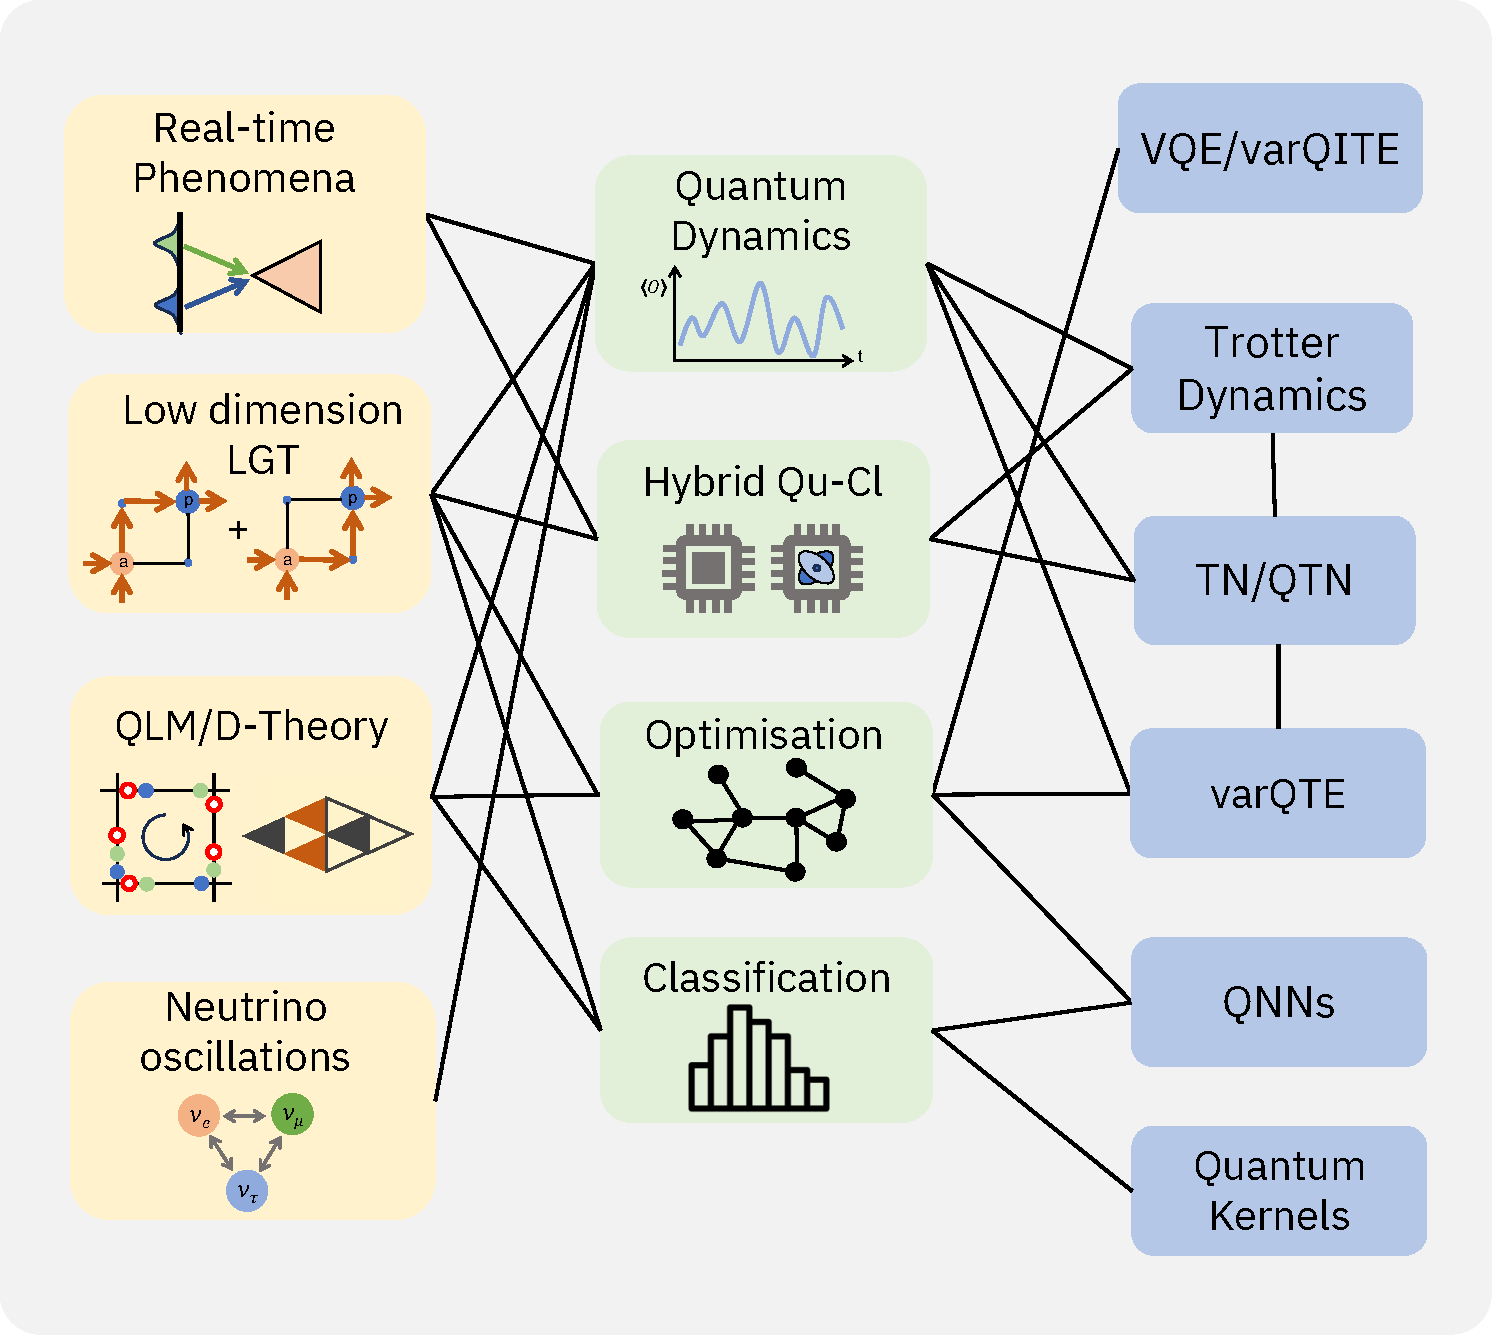
\includegraphics[width=.95 \columnwidth, keepaspectratio]{figures/Figure1a.pdf} \\
    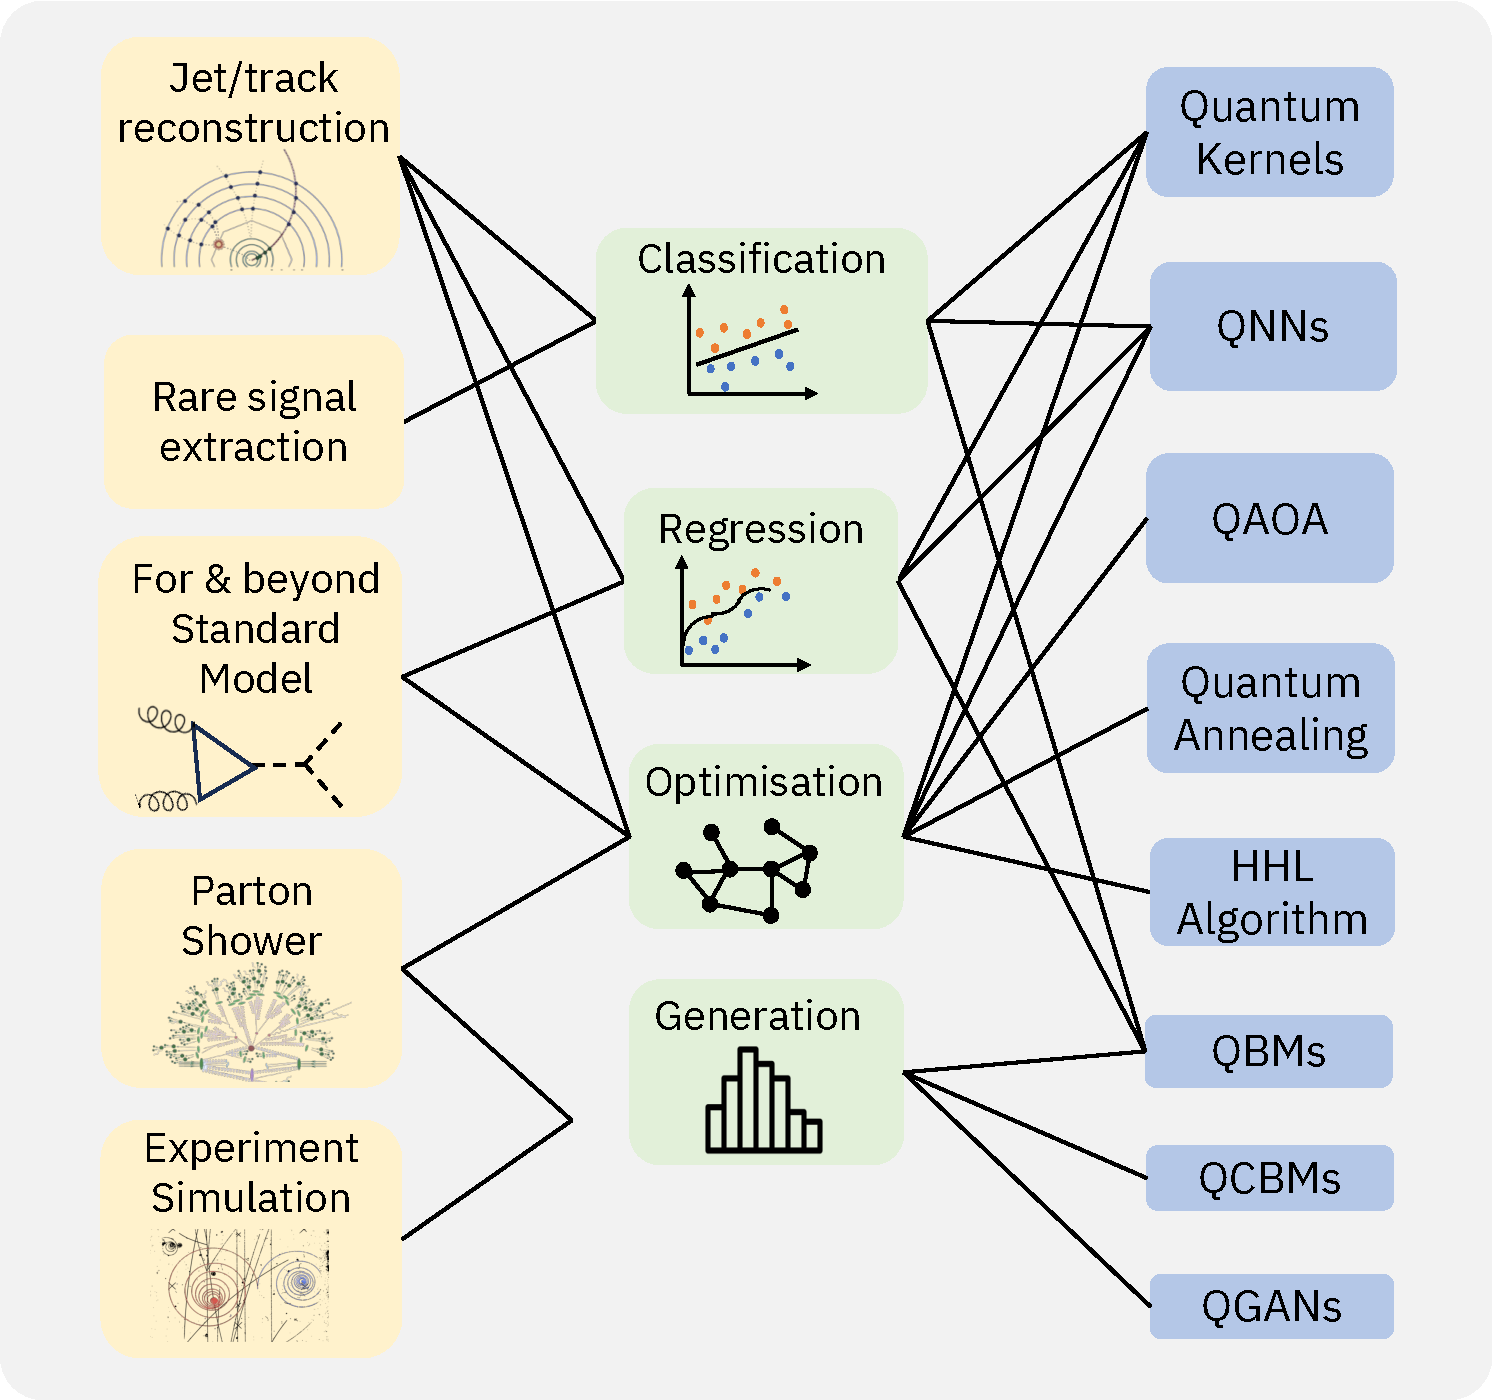
\includegraphics[width=.95 \columnwidth, keepaspectratio]{figures/Figure1b.pdf}
    \caption{(Upper Panel) Proposed theoretical physical model systems (orange) with corresponding approaches (green) and quantum algorithms (blue). For more information on the identified areas of interest see Section~\ref{subsect_Theory}. 
    (Lower Panel) 
    Proposed experimental challenges (orange) with corresponding approaches (green) and quantum algorithms (blue). For more information on the identified areas of interest see Section~\ref{subsect_Experiments}. 
    Legend: 
    VQE: Variational Eigensolver; 
    varQITE: variational Imaginary Time evolition;
    Tortter Dynamics: Time evolution based on trotteried time propagation operator;
    TN: Tensor Networks;
    QTN: Quantum Tensor Networks inspired from classical TN; 
    varQTE: variational Quantum Real Time evolution;
    QNN: Quantum Neural Networks;
    QAOA: Quantum Approximate Optimization Algorithm; 
    HHL Algorith:  Quantum algorithm for linear systems of equations (by Aram Harrow, Avinatan Hassidim, and Seth Lloyd);
    QBM: Quantum Boltzman Machines;
    QCBM: Quantum Circuit Born Machine; 
    QGANs: Quantum Generative Adversarial Networks.
    See Appendix~\ref{app:algos_limits} for an overview of a selection of these methods.}
    \label{fig:qiskit-merged}
\end{figure}


This article is organized as follows. In Sec.~\ref{sec:ibm_roadmap}, we outline IBM's roadmap for future quantum devices and explain why digital quantum computers are suitable for addressing open challenges in \gls{hep}. Subsequently we describe the challenges in the field and goals that are one hopes to achieve utilizing quantum hardware in Sec.~\ref{sec:goals}. Section~\ref{sec:algs} contains a description of various algorithms that we consider as key candidates for achieving the goals outlined in the previous section. Finally, we conclude in Sec.~\ref{sec:conclusion_outlook}. In appendix~\ref{appendix_resources}, we provide a detailed estimation of the required resources for encoding lattice gauge theories in a digital, qubit-based quantum computer, while appendix~\ref{app:algos_limits} contains information on selected quantum and classical algorithms.


\section{Classical simulation of quantum systems\label{sec:ClassicalSimulationOfQSystems}}

\subsection{Why use classical simulators}

For near-term quantum computers, one might question the necessity of classical simulators to emulate quantum computations. After all, the promise of quantum computing lies in its ability to perform certain tasks exponentially faster than classical computers. However, classical simulators remain invaluable for several compelling reasons \cite{10.1038/s41598-019-47174-9, 9910084,doi.org/10.48550,Fedorov2022unitaryselective,preopt-0,preopt-1,preopt-2,IBMQuantumSummit2023}.

\begin{enumerate}
    \item {\bf Resource Efficiency:} Quantum computer time is a limited and valuable resource. When developing and testing new quantum circuits or algorithms, researchers often need to execute them numerous times to validate their functionality and robustness. Running experiments on a real quantum machine can be time-consuming and costly, particularly when waiting for quantum computer availability after each circuit modification. Classical simulators offer an efficient alternative, allowing researchers to rapidly iterate through experiments without waiting for quantum resources.
    \item {\bf Noise and Error Analysis:} Real quantum machines are susceptible to noise and errors due to environmental factors, making it challenging to control and maintain the desired quantum state fidelity. Classical simulators provide a controlled environment for introducing and analyzing various noise scenarios. Researchers can simulate quantum noises to assess how robust their algorithms are under different conditions, as well as explore error correction techniques. This is a crucial step in building fault-tolerant quantum systems.
    \item {\bf Scalability:} Current quantum machines have limitations in terms of the number of qubits and the noise levels they exhibit. Classical simulators, on the other hand, can be adapted to simulate quantum systems with a larger number of qubits, enabling researchers to explore complex quantum algorithms and states that are beyond the capabilities of existing quantum hardware.
    \item {\bf Versatility:} Classical simulators offer flexibility regarding what they can simulate. Researchers can use them to capture "snapshots" of quantum states during computations, perform measurements, and make decisions based on measurement outcomes. Additionally, they can obtain more comprehensive information, such as the density operator of the system, rather than just specific measurement results.
    \item {\bf Efficiency Trade-Offs:} Building an efficient quantum simulator involves addressing trade-offs between computational efficiency and the range of quantum states it can represent. The choice of simulator depends on the specific needs of the quantum computation being emulated.
    \item {\bf Connectivity:}
    When executing a circuit on quantum hardware, the transpilation step involves mapping logical qubits to physical ones, in a fashion that may one-to-many. This is due to the constraint of the physical connection of qubits, which is not usually all-to-all on true QPUs. When simulating, all qubits can be entangled with all others, thus keeping down the `physical' qubits needed and easing the computational burden of solving the minor-embedding problem.
  \item {\bf Pre-optimization:}
    Variational algorithms can be expensive and require many iterations of a quantum circuit.  Pre-optimization with classical simulators can be used to find approximate circuits parameters that can be used or refined with quantum hardware.\cite{preopt-0,preopt-1,preopt-2}
    \item {\bf HPC-assisted quantum computing:}
    There is a way in which HPC can substantially help to extend the depth of quantum circuits, as demonstrated in the recently developed method called "Operator Backpropagation."~\cite{IBMQuantumSummit2023} The idea is to compute a part of a quantum circuit on a quantum device, and compute the second part of a circuit classically by using a quantum circuit simulator on an HPC system, and then stitch the results together. 
\end{enumerate}
In summary, classical simulators allow for efficient development, testing, and analysis of quantum circuits, algorithms, and states, while also providing a controlled environment for exploring quantum noise and errors. While quantum computers hold immense promise, classical simulators remain a vital component of the quantum computing toolkit, enabling progress and innovation in the field. Furthermore, simulators will likely continue to serve as yet another type of circuit execution environment among multi-node compute clusters for executing distributed workloads, which will be adept at handling (sub-)circuits that fall within their scope.

\subsection{Quantum circuits simulators}

In this section, we describe different types of classical quantum circuit simulators. In particular, we describe their capabilities in terms of what the maximum size systems (in both qubits and gates) that can be simulated using HPC. The advantages and disadvantages of quantum circuit simulators are also discussed, as well as use cases.

Before we start, we note that not every quantum circuit is difficult to simulate on a classical computer. Trivially, a quantum circuit that carries out a purely classical computation is not difficult to simulate on a classical computer. Indeed, some of the quantum circuits that are not difficult to simulate include Clifford circuits~\cite{gottesman1998heisenberg,aaronson2004improved,garcia2014simulation} and the quantum Fourier transform~\cite{aharonov2006quantum,yoran2007efficient}, to name a couple. Some quantum circuits are known to be classically simulable for specific input states as well~\cite{garcia2014simulation}. If the simulation does not need to produce the full spectrum of the output state of a given quantum computation but rather a sampling of such, as it would be the case for obtaining a final, classical result out of a quantum computer upon measurements, the difficulty of the classical simulation can dramatically decrease~\cite{hillmich2020just}. Further decrease in the difficulty is obtained if the simulation is to mimic an error-prone quantum computer executing a quantum circuit~\cite{hillmich2022approximating}. We further note in passing that simulation of a quantum circuit that exhibits sparse couplings between densely connected sets of qubits can be more amenable to classical simulations~\cite{fatima2021faster}, using methodologies not unlike circuit cutting discussed in Sec.~\ref{sec:CNA}.

\subsubsection{State-vector simulators}

State-vector based simulation is to simulate the operations of applying a series of unitary operators $U_{m-1} \cdots U_1 U_0$ to the state-vector representation of the quantum states $\ket{\psi}=\sum_{i=0}^{2^n-1}\alpha_i\ket{i}$, where $n$ is the number of qubits and $m$ is the number of operations or gates. Typically, a complex-valued double or single precision floating-point vector $\vec{\alpha}$ of size $2^n$ is used to store the coefficients $\alpha_i$, which costs $16\times2^n$ bytes of memory for classical simulation. $U_i$ with $i\in[0,m-1]$ is a $2\times2$ (for one-qubit gate) or $4\times4$ (for two-qubit gate) complex matrix. It has been shown that an arbitrary quantum circuit can be decomposed into 1-qubit and 2-qubit gates \cite{barenco1995elementary}. In fact, most quantum devices internally run 1-qubit or 2-qubit basis gates. For example, IBM adopts 1-qubit gate \texttt{X}, \texttt{SX}, \texttt{RZ}, \texttt{ID} and 2-qubit gate \texttt{CX} (recently \texttt{ECR}) as the basis gates. To apply a gate $U$, the operation is $\ket{\psi}\to U\ket{\psi}$. For 1-qubit $U$ applying on qubit $q$ in a quantum register, $\vec{\alpha}$ is updated through the following expression where $s_i=\lfloor i/{2^q}\rfloor 2^{q+1}+(i \% 2^q)$ for every integer $i\in[0, 2^{n-1}-1]$:
\begin{equation}
\begin{bmatrix}
\alpha_{s_i} \\
\alpha_{s_i+2^q}  
\end{bmatrix}
\to
U_{2\times2}\cdot \begin{bmatrix}
\alpha_{s_i} \\
\alpha_{s_i+2^q}  
\end{bmatrix}
\label{eq:1q-op}
\end{equation}
Regarding 2-qubit unitary gate $U$ applying on qubit $p$ and $q$ (assuming $p<q$ without losing generality), $\vec{\alpha}$ is updated  through:
\begin{equation}
\begin{bmatrix}
\alpha_{s_i} \\
\alpha_{s_i+2^p} \\
\alpha_{s_i+2^q} \\
\alpha_{s_i+2^p+2^q}
\end{bmatrix}
\to
U_{4\times4}\cdot \begin{bmatrix}
\alpha_{s_i} \\
\alpha_{s_i+2^p} \\
\alpha_{s_i+2^q} \\
\alpha_{s_i+2^p+2^q}
\end{bmatrix}
\label{eq:2q-op}
\end{equation}
where $s_i{=}\lfloor \lfloor i/{2^p}\rfloor /2^{q-p-1} \rfloor  2^{q+1} + (\lfloor i/{2^p}\rfloor \% 2^{q-p-1})2^{p+1} +  (i \% 2^p)$ for every integer $i\in[0,2^{n-2}-1]$. 

Therefore, state-vector based quantum numerical simulation is to perform a sequence of $2\times2$ or $4\times4$ operations Eq.~(\ref{eq:1q-op}) and Eq.~(\ref{eq:2q-op}) over the large state-vector coefficient array of complex numbers in a classical system.

State vector simulators hold the full coefficients of pure quantum states within the classical system's memory, which scales exponentially with the number of qubits. Consequently, the state vector is often distributed across many nodes of a classical HPC~\cite{haner20170,pednault2017breaking,pednault2019leveraging,li2021sv}. Such simulators however exhibit linear scaling with respect to the circuit depth~\cite{fatima2021faster}. As such, state vector simulations are sensitive to the number of qubits but much less to the gate count or circuit depth. For example, a recent work shows that a low-energy nuclear quantum circuit with 115 million gates on 21-qubits can be effectively simulated within one hour using a GPU for state vector simulation~\cite{li2023deep}.

We note that various forms of approximate state-vector simulators can be tailored to problem specific applications.  For example, recent truncated state vector simulators have been used to simulate VQE for various chemistry problems on 64 qubits without significant loss of accuracy or the need for large computing resources~\cite{preopt-2,approxstatevec}. Combining the state vector simulators with Feynman path summation can trade the circuit depth with the number of qubits or memory usage~\cite{fatima2021faster}, rendering some hard to simulate circuits according to a naive state vector simulator to be simulable due to orders of magnitude improvement in their simulability~\cite{markov2020massively,fatima2021faster}.

\subsubsection{Density matrix simulators}

When dealing with a mixed system where noise is present, a pure state can no longer provide sufficient information about the system. In this case, a mixed state corresponds to a statistical ensemble, or probabilistic mixture of pure states, can be used to describe the condition where a system is entangled with another system, such as the environment from which the noise is imposed. A mixed state is represented by a density matrix or a density operator, which is defined by choosing the basis in the underlying space. The density matrix is given by:
\begin{equation*}
\rho=\sum{p_s\ket{\psi_s}\bra{\psi_s}}
\end{equation*}
where $\rho$ represents the fraction of the ensemble of each pure state and is generally an unknown real value. A density matrix contains all the information of a quantum system, allowing the calculation of the probabilities of the outcomes of any measurement performed.

Compared to state-vector simulation, the density operator requires the conservation of $4^n$ coefficients, where $n$ is the number of eigenstates for each pure state, i.e., the number of qubits. Therefore, the memory cost of a density matrix simulation is $2^n$ times that of a pure state simulation using state-vector. The system also evolves according to the operator or gate sequence. When a particular gate is applied, the density matrix evolves as follows~\cite{li2020density}:
\begin{equation}
\rho(t)=G(t)\rho(0)G(t)^{\dagger}
 \label{eq:onegate}
\end{equation}
where $G(t)$ is the gate at time $t$, and $G(t)^\dagger$ is its adjoint. The evolution of a density matrix is more complicated than that of a state vector, considering the size of $4^n$ and the extra adjoint operator per gate. Although $G(t)$ by itself is a unitary operator, it becomes a general matrix and is not necessarily unitary in the presence of noise. Depending on the noise model, the evolution can become an ensemble of evolutions of corresponding channels, each described by a Kraus operator.

The noisy density matrix quantum numerical simulation is to compute $\rho_\text{out}$ for a n-qubit quantum system, density matrix quantum circuit simulation is to compute $\rho_\text{out}$ for a n-qubit quantum register, given initial state $\rho_\text{in}$ and $m$ non-unitary transformations $G_0$, $G_1$, $\dots$, $G_{m-1}$:
\begin{equation}
 \rho_{\text{out}} = G_{m-1}\cdots (G_1 (G_0 \rho_{\text{in}} G^\dag_0) G^\dag_1)\cdots G^\dag_{m-1}
 \label{eq:dmsim}
\end{equation}
where $G$ and $\rho$ are $2^n\times 2^n$ matrices. Due to noise, $G$ is not necessarily a unitary matrix. $G^\dag$ is the adjoint of $G$ verifying $G^\dag=(G^*)^T$. As real quantum devices typically use 1-qubit or 2-qubit gates representing as $4\times4$ or $16\times16$ matrices, to obtain the matrix $G_i$ with a $2^n\times2^n$ size, Kronecker product or tensor product is used with the identity matrix $I$ for the other qubits. 


\subsubsection{Tensor network simulators}

Quantum tensor networks can be used for the simulation of quantum circuits~\cite{markov2008simulating, lykov2021importance, lykov2021large, lykov2021performance, lykov2022tensor, berquist2022stochastic, shah2023gpu}. These simulators leverage the mathematical framework of tensor networks, which are graphical representations of quantum states and operations, as networks of interconnected tensors. Specifially, the nodes in these networks correspond to tensors, which encode gate operations, while the edges represent indices along which tensors are contracted, reflecting the entanglement and interactions between qubits.

The strength of tensor network simulators lies in their ability to compactly represent quantum states that would otherwise require a prohibitive amount of memory. This is particularly valuable for simulating shallow-depth quantum circuits with a large number of qubits, which are challenging for traditional state-vector simulators. These simulators are still limited by the amount of available distributed memory on a supercomputer. For the current generation of supercomputers, tensor network simulators can run quantum circuits up to approximately 200 qubits without approximations for certain quantum circuits~\cite{lykov2021large}. Larger simulations are possible with a truncated bond dimension as well as other applications with different resource requirements~\cite{preopt-1}.


There are different types of tensor network simulators: Matrix Product States (MPS), Projected Entangled Pair States (PEPS), Tree Tensor Networks (TTN), Multi-scale Entanglement Renormalization Ansatz (MERA), and Continuous Variable Tensor Network (CVTN) to name a few as shown on Figure~\ref{fig:tensornetworks}. MPS is arguably one of the most popular simulators, and it is particularly useful for simulating one-dimensional quantum systems. In MPS, the tensors are arranged in a chain, with each tensor representing the state of a qubit and the connections between them capturing the nearest-neighbor entanglement. One of the MPS applications is an efficient tensor network simulation of lossy Gaussian boson sampling experiments, which has been recently demonstrated \cite{liu2023simulating, Oh2023}.
%{\color{red}Minh: Can we briefly comment on when the other methods (PEPS, TTN, ...) are good?}

\begin{figure}
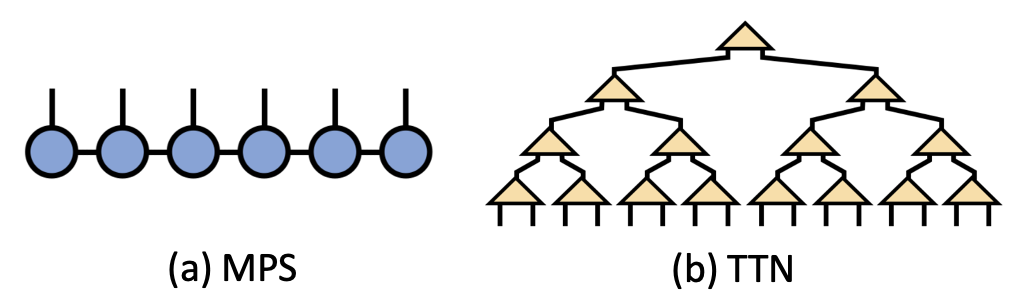
\includegraphics[width=\columnwidth]{groups/3._Classical_simulation_of_quantum_systems/MPS-TTN.png}
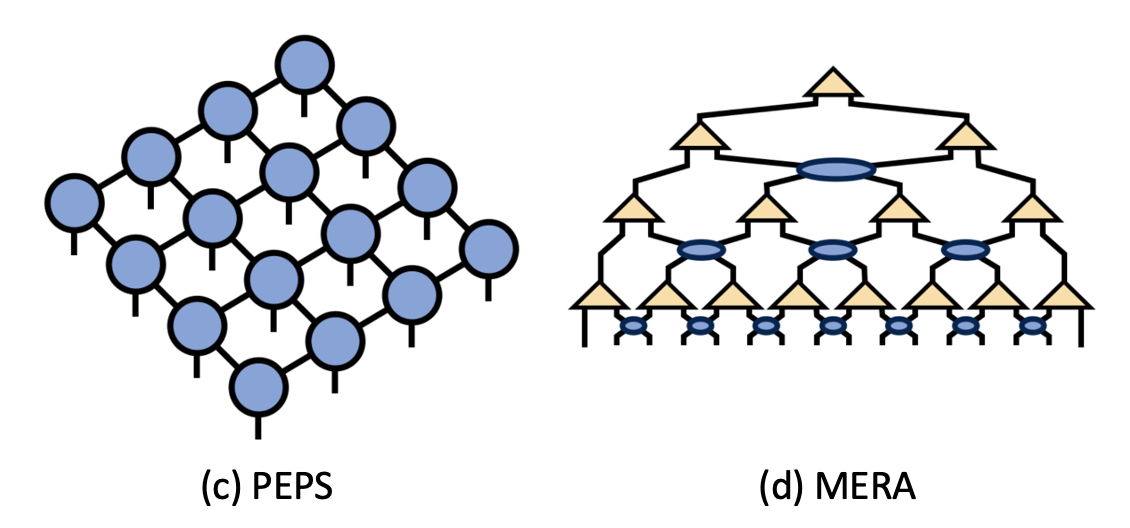
\includegraphics[width=\columnwidth]{groups/3._Classical_simulation_of_quantum_systems/PEPS-MERA.png}
\caption{Different types of tensor network simulators: (a) Matrix Product States (MPS), (b) Tree Tensor Networks (TTN), (c) Projected Entangled Pair States (PEPS), and (d) Multi-scale Entanglement Renormalization Ansatz (MERA).}
\label{fig:tensornetworks}
\end{figure}

Each type of tensor network has its specific applications, advantages, and limitations, and the choice of which to use depends on the application, size, and structure of a quantum circuit:
\begin{itemize}
    
\item MPS simulators excel in one-dimensional quantum systems with short-range interactions. They are efficient for simulating ground and excited states, as well as dynamical properties, due to their ability to capture entanglement in a scalable manner with limited entanglement entropy.

\item  PEPS are generalizations of MPS to higher dimensions, making them suitable for two-dimensional quantum systems. They are adept at handling both short- and long-range interactions, but their computational complexity increases significantly with the system's size and entanglement.

\item  TTN simulators are structured in a hierarchical, tree-like manner, offering efficient computation for certain quantum circuits, especially those with hierarchical or layered structures. They are particularly useful for simulating states that exhibit hierarchical entanglement patterns and for providing insights into quantum many-body systems.

\item  MERA is designed for critical systems with long-range entanglement. It excels in representing ground states of quantum many-body systems near criticality, offering insights into scaling and universality in quantum phase transitions.

\item  CTVN simulators are tailored for quantum systems with continuous variables, like quantum fields or modes of light. They are adept at handling systems where particle number isn't conserved and are crucial in studying non-Gaussian states and processes in quantum optics and field theories.
\end{itemize}

Tensor network simulators continue to evolve, with ongoing research aimed at increasing their efficiency, scalability, and applicability to a broader range of quantum computing tasks.


\subsubsection{Open system Lindblad quantum simulators}

Open-system Lindblad quantum simulators are specifically designed to model the dynamics of quantum systems interacting with external environments. The applications include, for example, simulating quantum magnetism, topological materials, 
quantum phase transitions, and electron transportation. Unlike closed quantum systems, open systems are subject to environmental influences that lead to non-unitary processes such as decoherence and dissipation. These simulators leverage the Lindblad master equation, which blends the unitary evolution dictated by the system's Hamiltonian with the non-unitary aspects resulting from environmental interactions. This approach allows for a comprehensive simulation of open quantum systems, capturing the complexity of quantum noise and the environmental effects. Recently, a novel approach, called noisy quantum gates, has been proposed, as a classical simulation of the Lindblad dynamics~\cite{noisygates}. It is based on integrating the noise into the gates, rather than keeping gates and noise as two separate dynamics, an approach can be generalized to non-Markovian dynamics by using colored noises.

In general, there are a few ways to formulate, but the most common is to use the density matrix formalism, which is adept at representing mixed states, a critical aspect when dealing with open systems. These simulators provide researchers with the flexibility to define specific system-environment interactions, making them a versatile tool across various quantum research domains, especially in material science applications. Its ability to accurately model quantum noise induced by the environment is an especially valuable aspect of it. Overall, the open-system Lindblad quantum simulators stand as a very valuable tool in quantum research, enabling a deeper understanding of the environmental impacts on quantum systems and aiding in the advancement of practical quantum applications.


\subsection{Overview of classical simulators}

In summary, we described four main types of quantum circuit simulators. In the context of material science, the choice of a quantum circuit simulator depends on the specific characteristics of the system under study and the phenomena of interest. Here is how each type of simulator can be used:

State-vector simulators are ideal for systems that can be accurately represented by pure quantum states. In material science, they are particularly useful for studying the evolution of quantum states under Hamiltonians with relatively few degrees of freedom. They excel in scenarios where the full quantum state needs to be tracked, such as in the simulation of small, isolated quantum systems or systems with limited entanglement.

Density matrix simulators are well suited for studying systems where mixed states are prevalent, which includes most real-world scenarios in material science. They can handle decoherence and other noise effects, making them suitable for simulating open quantum systems or systems under non-ideal conditions. Density matrix simulators are ideal for investigating phenomena in quantum materials where environmental interactions play a significant role.

Different types of tensor network simulators have different use cases.
MPS and TTN are powerful in simulating one-dimensional and certain hierarchical quantum systems, respectively. They can efficiently model systems with short-range interactions, which are common in material science. These simulators are especially useful for studying ground state properties and low-energy excitations in materials.
PEPS and MERA are more suited for higher-dimensional systems. PEPS can handle both short- and long-range interactions in two-dimensional materials, making them valuable for exploring complex quantum materials, such as high-temperature superconductors. MERA is particularly effective in studying critical phenomena and phase transitions in materials.

Open system Lindblad quantum simulators are designed to handle non-unitary evolution, which is typical in open quantum systems, where the system is in contact with an external environment. In material science, they are crucial for studying decoherence, dissipation, and thermalization processes in materials. Lindblad simulators are particularly relevant for investigating quantum materials and devices operating under realistic, non-ideal conditions, where environmental interactions cannot be ignored. They are essential for understanding the behavior of materials in quantum information processing and quantum sensing applications, where control and mitigation of decoherence are critical.

Using HPC is critical for simulating large quantum circuits. Ultimately, supercomputers can simulate relatively small quantum circuits because of the exponential requirement of available distributed memory. The next generation of quantum simulators will probably use small quantum computers to simulate very large quantum circuits. The idea is to use small quantum computers to perform tasks that are inherently quantum in nature, such as the contraction of intermediate multi-dimensional tensors, which are central to tensor network simulations. This idea is closely related to Feynman's proposal to use quantum computers to simulate quantum systems~\cite{hey2018feynman}. One way is to use Harrow-Hassidim-Lloyd (HHL) algorithm for the contraction of very high-dimension tensors, which is currently a bottleneck of classical tensor network simulators. The HHL algorithm can be adapted to perform tensor contractions by encoding the tensors as linear systems. This could potentially revolutionize tensor network simulations by dramatically reducing the computational complexity of these contractions. This approach promises a scalable pathway for quantum simulation, as improvements in quantum hardware, such as increased qubit counts and enhanced coherence times, would directly translate into an increased capacity for simulating larger and more complex quantum circuits.

\iffalse
\subsection{Simulation of time dynamics} 
Move to another section.

People: Yuri Alexeev, Burns Healy, Bo Phang, Niri Govind

Describe here the challenges of simulating time dynamics classically and make the case for quantum simulations. Cover topics such as simulation of quantum effects, scalability, and accuracy.

Write text on Yang-Baxter circuit compression. Describe how to perform these calculations efficiently and the challenges for achieving quantum advantage.

The time evolution of quantum systems described by Ising-type Hamiltonians is a very important problem in condensed matter physics and quantum information. These Hamiltonians encompass a wide range of physical phenomena, from magnetic interactions in condensed matter systems to the formulation of optimization problems for quantum computing. In particular, the Ising model describes a lattice of spins with pairwise interactions, characterized by a Hamiltonian that depends on the arrangement of spins and the interaction strengths between them. The general form of an Ising-type Hamiltonian is given by:

\begin{equation}
H = -\sum_{i, j} J_{ij}(t) \sigma_i \sigma_j - \sum_{i} h_i(t) \sigma_i,
\label{ising_hamiltonian}
\end{equation}

where $\sigma_i^z$ and $\sigma_i^x$ represent Pauli matrices, $J_{ij}(t)$ are time-dependent coupling strengths, $h_i(t)$ are time-dependent magnetic fields, and the summations extend over all pairs of spins and single-spin terms.

The problem of accurate large-scale time dynamics simulations remains an area of active research. List the challenges (noise, size, time dynamics length) and opportunities.


\subsection{Simulation of ground states}

Quantum Monte Carlo, etc. 

\subsection{Simulation of finite-temperature systems}

\fi









\section{Classical simulation of quantum systems\label{sec:ClassicalSimulationOfQSystems}}

\subsection{Why use classical simulators}

For near-term quantum computers, one might question the necessity of classical simulators to emulate quantum computations. After all, the promise of quantum computing lies in its ability to perform certain tasks exponentially faster than classical computers. However, classical simulators remain invaluable for several compelling reasons \cite{10.1038/s41598-019-47174-9, 9910084,doi.org/10.48550,Fedorov2022unitaryselective,preopt-0,preopt-1,preopt-2,IBMQuantumSummit2023}.

\begin{enumerate}
    \item {\bf Resource Efficiency:} Quantum computer time is a limited and valuable resource. When developing and testing new quantum circuits or algorithms, researchers often need to execute them numerous times to validate their functionality and robustness. Running experiments on a real quantum machine can be time-consuming and costly, particularly when waiting for quantum computer availability after each circuit modification. Classical simulators offer an efficient alternative, allowing researchers to rapidly iterate through experiments without waiting for quantum resources.
    \item {\bf Noise and Error Analysis:} Real quantum machines are susceptible to noise and errors due to environmental factors, making it challenging to control and maintain the desired quantum state fidelity. Classical simulators provide a controlled environment for introducing and analyzing various noise scenarios. Researchers can simulate quantum noises to assess how robust their algorithms are under different conditions, as well as explore error correction techniques. This is a crucial step in building fault-tolerant quantum systems.
    \item {\bf Scalability:} Current quantum machines have limitations in terms of the number of qubits and the noise levels they exhibit. Classical simulators, on the other hand, can be adapted to simulate quantum systems with a larger number of qubits, enabling researchers to explore complex quantum algorithms and states that are beyond the capabilities of existing quantum hardware.
    \item {\bf Versatility:} Classical simulators offer flexibility regarding what they can simulate. Researchers can use them to capture "snapshots" of quantum states during computations, perform measurements, and make decisions based on measurement outcomes. Additionally, they can obtain more comprehensive information, such as the density operator of the system, rather than just specific measurement results.
    \item {\bf Efficiency Trade-Offs:} Building an efficient quantum simulator involves addressing trade-offs between computational efficiency and the range of quantum states it can represent. The choice of simulator depends on the specific needs of the quantum computation being emulated.
    \item {\bf Connectivity:}
    When executing a circuit on quantum hardware, the transpilation step involves mapping logical qubits to physical ones, in a fashion that may one-to-many. This is due to the constraint of the physical connection of qubits, which is not usually all-to-all on true QPUs. When simulating, all qubits can be entangled with all others, thus keeping down the `physical' qubits needed and easing the computational burden of solving the minor-embedding problem.
  \item {\bf Pre-optimization:}
    Variational algorithms can be expensive and require many iterations of a quantum circuit.  Pre-optimization with classical simulators can be used to find approximate circuits parameters that can be used or refined with quantum hardware.\cite{preopt-0,preopt-1,preopt-2}
    \item {\bf HPC-assisted quantum computing:}
    There is a way in which HPC can substantially help to extend the depth of quantum circuits, as demonstrated in the recently developed method called "Operator Backpropagation."~\cite{IBMQuantumSummit2023} The idea is to compute a part of a quantum circuit on a quantum device, and compute the second part of a circuit classically by using a quantum circuit simulator on an HPC system, and then stitch the results together. 
\end{enumerate}
In summary, classical simulators allow for efficient development, testing, and analysis of quantum circuits, algorithms, and states, while also providing a controlled environment for exploring quantum noise and errors. While quantum computers hold immense promise, classical simulators remain a vital component of the quantum computing toolkit, enabling progress and innovation in the field. Furthermore, simulators will likely continue to serve as yet another type of circuit execution environment among multi-node compute clusters for executing distributed workloads, which will be adept at handling (sub-)circuits that fall within their scope.

\subsection{Quantum circuits simulators}

In this section, we describe different types of classical quantum circuit simulators. In particular, we describe their capabilities in terms of what the maximum size systems (in both qubits and gates) that can be simulated using HPC. The advantages and disadvantages of quantum circuit simulators are also discussed, as well as use cases.

Before we start, we note that not every quantum circuit is difficult to simulate on a classical computer. Trivially, a quantum circuit that carries out a purely classical computation is not difficult to simulate on a classical computer. Indeed, some of the quantum circuits that are not difficult to simulate include Clifford circuits~\cite{gottesman1998heisenberg,aaronson2004improved,garcia2014simulation} and the quantum Fourier transform~\cite{aharonov2006quantum,yoran2007efficient}, to name a couple. Some quantum circuits are known to be classically simulable for specific input states as well~\cite{garcia2014simulation}. If the simulation does not need to produce the full spectrum of the output state of a given quantum computation but rather a sampling of such, as it would be the case for obtaining a final, classical result out of a quantum computer upon measurements, the difficulty of the classical simulation can dramatically decrease~\cite{hillmich2020just}. Further decrease in the difficulty is obtained if the simulation is to mimic an error-prone quantum computer executing a quantum circuit~\cite{hillmich2022approximating}. We further note in passing that simulation of a quantum circuit that exhibits sparse couplings between densely connected sets of qubits can be more amenable to classical simulations~\cite{fatima2021faster}, using methodologies not unlike circuit cutting discussed in Sec.~\ref{sec:CNA}.

\subsubsection{State-vector simulators}

State-vector based simulation is to simulate the operations of applying a series of unitary operators $U_{m-1} \cdots U_1 U_0$ to the state-vector representation of the quantum states $\ket{\psi}=\sum_{i=0}^{2^n-1}\alpha_i\ket{i}$, where $n$ is the number of qubits and $m$ is the number of operations or gates. Typically, a complex-valued double or single precision floating-point vector $\vec{\alpha}$ of size $2^n$ is used to store the coefficients $\alpha_i$, which costs $16\times2^n$ bytes of memory for classical simulation. $U_i$ with $i\in[0,m-1]$ is a $2\times2$ (for one-qubit gate) or $4\times4$ (for two-qubit gate) complex matrix. It has been shown that an arbitrary quantum circuit can be decomposed into 1-qubit and 2-qubit gates \cite{barenco1995elementary}. In fact, most quantum devices internally run 1-qubit or 2-qubit basis gates. For example, IBM adopts 1-qubit gate \texttt{X}, \texttt{SX}, \texttt{RZ}, \texttt{ID} and 2-qubit gate \texttt{CX} (recently \texttt{ECR}) as the basis gates. To apply a gate $U$, the operation is $\ket{\psi}\to U\ket{\psi}$. For 1-qubit $U$ applying on qubit $q$ in a quantum register, $\vec{\alpha}$ is updated through the following expression where $s_i=\lfloor i/{2^q}\rfloor 2^{q+1}+(i \% 2^q)$ for every integer $i\in[0, 2^{n-1}-1]$:
\begin{equation}
\begin{bmatrix}
\alpha_{s_i} \\
\alpha_{s_i+2^q}  
\end{bmatrix}
\to
U_{2\times2}\cdot \begin{bmatrix}
\alpha_{s_i} \\
\alpha_{s_i+2^q}  
\end{bmatrix}
\label{eq:1q-op}
\end{equation}
Regarding 2-qubit unitary gate $U$ applying on qubit $p$ and $q$ (assuming $p<q$ without losing generality), $\vec{\alpha}$ is updated  through:
\begin{equation}
\begin{bmatrix}
\alpha_{s_i} \\
\alpha_{s_i+2^p} \\
\alpha_{s_i+2^q} \\
\alpha_{s_i+2^p+2^q}
\end{bmatrix}
\to
U_{4\times4}\cdot \begin{bmatrix}
\alpha_{s_i} \\
\alpha_{s_i+2^p} \\
\alpha_{s_i+2^q} \\
\alpha_{s_i+2^p+2^q}
\end{bmatrix}
\label{eq:2q-op}
\end{equation}
where $s_i{=}\lfloor \lfloor i/{2^p}\rfloor /2^{q-p-1} \rfloor  2^{q+1} + (\lfloor i/{2^p}\rfloor \% 2^{q-p-1})2^{p+1} +  (i \% 2^p)$ for every integer $i\in[0,2^{n-2}-1]$. 

Therefore, state-vector based quantum numerical simulation is to perform a sequence of $2\times2$ or $4\times4$ operations Eq.~(\ref{eq:1q-op}) and Eq.~(\ref{eq:2q-op}) over the large state-vector coefficient array of complex numbers in a classical system.

State vector simulators hold the full coefficients of pure quantum states within the classical system's memory, which scales exponentially with the number of qubits. Consequently, the state vector is often distributed across many nodes of a classical HPC~\cite{haner20170,pednault2017breaking,pednault2019leveraging,li2021sv}. Such simulators however exhibit linear scaling with respect to the circuit depth~\cite{fatima2021faster}. As such, state vector simulations are sensitive to the number of qubits but much less to the gate count or circuit depth. For example, a recent work shows that a low-energy nuclear quantum circuit with 115 million gates on 21-qubits can be effectively simulated within one hour using a GPU for state vector simulation~\cite{li2023deep}.

We note that various forms of approximate state-vector simulators can be tailored to problem specific applications.  For example, recent truncated state vector simulators have been used to simulate VQE for various chemistry problems on 64 qubits without significant loss of accuracy or the need for large computing resources~\cite{preopt-2,approxstatevec}. Combining the state vector simulators with Feynman path summation can trade the circuit depth with the number of qubits or memory usage~\cite{fatima2021faster}, rendering some hard to simulate circuits according to a naive state vector simulator to be simulable due to orders of magnitude improvement in their simulability~\cite{markov2020massively,fatima2021faster}.

\subsubsection{Density matrix simulators}

When dealing with a mixed system where noise is present, a pure state can no longer provide sufficient information about the system. In this case, a mixed state corresponds to a statistical ensemble, or probabilistic mixture of pure states, can be used to describe the condition where a system is entangled with another system, such as the environment from which the noise is imposed. A mixed state is represented by a density matrix or a density operator, which is defined by choosing the basis in the underlying space. The density matrix is given by:
\begin{equation*}
\rho=\sum{p_s\ket{\psi_s}\bra{\psi_s}}
\end{equation*}
where $\rho$ represents the fraction of the ensemble of each pure state and is generally an unknown real value. A density matrix contains all the information of a quantum system, allowing the calculation of the probabilities of the outcomes of any measurement performed.

Compared to state-vector simulation, the density operator requires the conservation of $4^n$ coefficients, where $n$ is the number of eigenstates for each pure state, i.e., the number of qubits. Therefore, the memory cost of a density matrix simulation is $2^n$ times that of a pure state simulation using state-vector. The system also evolves according to the operator or gate sequence. When a particular gate is applied, the density matrix evolves as follows~\cite{li2020density}:
\begin{equation}
\rho(t)=G(t)\rho(0)G(t)^{\dagger}
 \label{eq:onegate}
\end{equation}
where $G(t)$ is the gate at time $t$, and $G(t)^\dagger$ is its adjoint. The evolution of a density matrix is more complicated than that of a state vector, considering the size of $4^n$ and the extra adjoint operator per gate. Although $G(t)$ by itself is a unitary operator, it becomes a general matrix and is not necessarily unitary in the presence of noise. Depending on the noise model, the evolution can become an ensemble of evolutions of corresponding channels, each described by a Kraus operator.

The noisy density matrix quantum numerical simulation is to compute $\rho_\text{out}$ for a n-qubit quantum system, density matrix quantum circuit simulation is to compute $\rho_\text{out}$ for a n-qubit quantum register, given initial state $\rho_\text{in}$ and $m$ non-unitary transformations $G_0$, $G_1$, $\dots$, $G_{m-1}$:
\begin{equation}
 \rho_{\text{out}} = G_{m-1}\cdots (G_1 (G_0 \rho_{\text{in}} G^\dag_0) G^\dag_1)\cdots G^\dag_{m-1}
 \label{eq:dmsim}
\end{equation}
where $G$ and $\rho$ are $2^n\times 2^n$ matrices. Due to noise, $G$ is not necessarily a unitary matrix. $G^\dag$ is the adjoint of $G$ verifying $G^\dag=(G^*)^T$. As real quantum devices typically use 1-qubit or 2-qubit gates representing as $4\times4$ or $16\times16$ matrices, to obtain the matrix $G_i$ with a $2^n\times2^n$ size, Kronecker product or tensor product is used with the identity matrix $I$ for the other qubits. 


\subsubsection{Tensor network simulators}

Quantum tensor networks can be used for the simulation of quantum circuits~\cite{markov2008simulating, lykov2021importance, lykov2021large, lykov2021performance, lykov2022tensor, berquist2022stochastic, shah2023gpu}. These simulators leverage the mathematical framework of tensor networks, which are graphical representations of quantum states and operations, as networks of interconnected tensors. Specifially, the nodes in these networks correspond to tensors, which encode gate operations, while the edges represent indices along which tensors are contracted, reflecting the entanglement and interactions between qubits.

The strength of tensor network simulators lies in their ability to compactly represent quantum states that would otherwise require a prohibitive amount of memory. This is particularly valuable for simulating shallow-depth quantum circuits with a large number of qubits, which are challenging for traditional state-vector simulators. These simulators are still limited by the amount of available distributed memory on a supercomputer. For the current generation of supercomputers, tensor network simulators can run quantum circuits up to approximately 200 qubits without approximations for certain quantum circuits~\cite{lykov2021large}. Larger simulations are possible with a truncated bond dimension as well as other applications with different resource requirements~\cite{preopt-1}.


There are different types of tensor network simulators: Matrix Product States (MPS), Projected Entangled Pair States (PEPS), Tree Tensor Networks (TTN), Multi-scale Entanglement Renormalization Ansatz (MERA), and Continuous Variable Tensor Network (CVTN) to name a few as shown on Figure~\ref{fig:tensornetworks}. MPS is arguably one of the most popular simulators, and it is particularly useful for simulating one-dimensional quantum systems. In MPS, the tensors are arranged in a chain, with each tensor representing the state of a qubit and the connections between them capturing the nearest-neighbor entanglement. One of the MPS applications is an efficient tensor network simulation of lossy Gaussian boson sampling experiments, which has been recently demonstrated \cite{liu2023simulating, Oh2023}.
%{\color{red}Minh: Can we briefly comment on when the other methods (PEPS, TTN, ...) are good?}

\begin{figure}
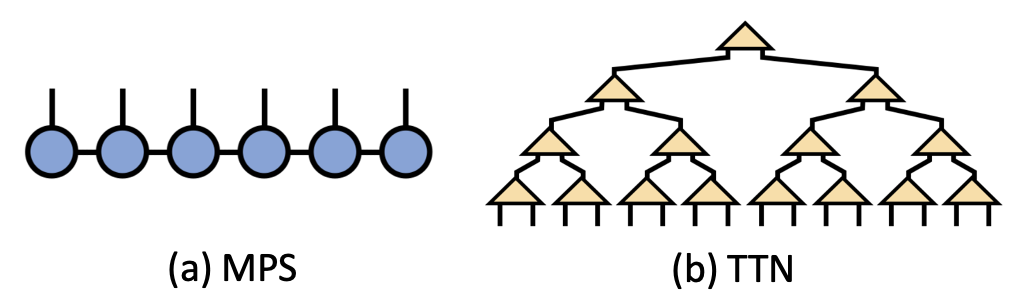
\includegraphics[width=\columnwidth]{groups/3._Classical_simulation_of_quantum_systems/MPS-TTN.png}
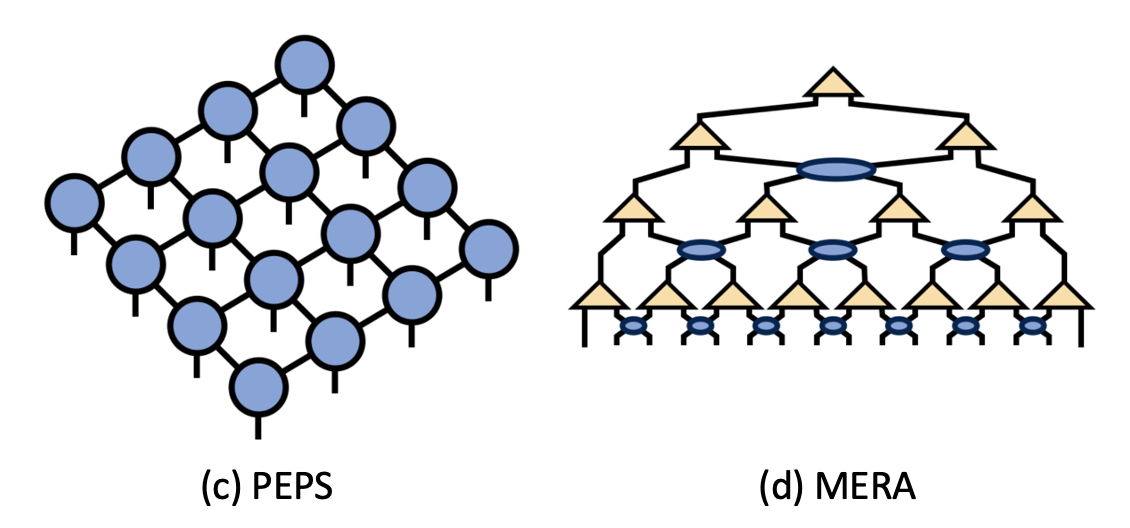
\includegraphics[width=\columnwidth]{groups/3._Classical_simulation_of_quantum_systems/PEPS-MERA.png}
\caption{Different types of tensor network simulators: (a) Matrix Product States (MPS), (b) Tree Tensor Networks (TTN), (c) Projected Entangled Pair States (PEPS), and (d) Multi-scale Entanglement Renormalization Ansatz (MERA).}
\label{fig:tensornetworks}
\end{figure}

Each type of tensor network has its specific applications, advantages, and limitations, and the choice of which to use depends on the application, size, and structure of a quantum circuit:
\begin{itemize}
    
\item MPS simulators excel in one-dimensional quantum systems with short-range interactions. They are efficient for simulating ground and excited states, as well as dynamical properties, due to their ability to capture entanglement in a scalable manner with limited entanglement entropy.

\item  PEPS are generalizations of MPS to higher dimensions, making them suitable for two-dimensional quantum systems. They are adept at handling both short- and long-range interactions, but their computational complexity increases significantly with the system's size and entanglement.

\item  TTN simulators are structured in a hierarchical, tree-like manner, offering efficient computation for certain quantum circuits, especially those with hierarchical or layered structures. They are particularly useful for simulating states that exhibit hierarchical entanglement patterns and for providing insights into quantum many-body systems.

\item  MERA is designed for critical systems with long-range entanglement. It excels in representing ground states of quantum many-body systems near criticality, offering insights into scaling and universality in quantum phase transitions.

\item  CTVN simulators are tailored for quantum systems with continuous variables, like quantum fields or modes of light. They are adept at handling systems where particle number isn't conserved and are crucial in studying non-Gaussian states and processes in quantum optics and field theories.
\end{itemize}

Tensor network simulators continue to evolve, with ongoing research aimed at increasing their efficiency, scalability, and applicability to a broader range of quantum computing tasks.


\subsubsection{Open system Lindblad quantum simulators}

Open-system Lindblad quantum simulators are specifically designed to model the dynamics of quantum systems interacting with external environments. The applications include, for example, simulating quantum magnetism, topological materials, 
quantum phase transitions, and electron transportation. Unlike closed quantum systems, open systems are subject to environmental influences that lead to non-unitary processes such as decoherence and dissipation. These simulators leverage the Lindblad master equation, which blends the unitary evolution dictated by the system's Hamiltonian with the non-unitary aspects resulting from environmental interactions. This approach allows for a comprehensive simulation of open quantum systems, capturing the complexity of quantum noise and the environmental effects. Recently, a novel approach, called noisy quantum gates, has been proposed, as a classical simulation of the Lindblad dynamics~\cite{noisygates}. It is based on integrating the noise into the gates, rather than keeping gates and noise as two separate dynamics, an approach can be generalized to non-Markovian dynamics by using colored noises.

In general, there are a few ways to formulate, but the most common is to use the density matrix formalism, which is adept at representing mixed states, a critical aspect when dealing with open systems. These simulators provide researchers with the flexibility to define specific system-environment interactions, making them a versatile tool across various quantum research domains, especially in material science applications. Its ability to accurately model quantum noise induced by the environment is an especially valuable aspect of it. Overall, the open-system Lindblad quantum simulators stand as a very valuable tool in quantum research, enabling a deeper understanding of the environmental impacts on quantum systems and aiding in the advancement of practical quantum applications.


\subsection{Overview of classical simulators}

In summary, we described four main types of quantum circuit simulators. In the context of material science, the choice of a quantum circuit simulator depends on the specific characteristics of the system under study and the phenomena of interest. Here is how each type of simulator can be used:

State-vector simulators are ideal for systems that can be accurately represented by pure quantum states. In material science, they are particularly useful for studying the evolution of quantum states under Hamiltonians with relatively few degrees of freedom. They excel in scenarios where the full quantum state needs to be tracked, such as in the simulation of small, isolated quantum systems or systems with limited entanglement.

Density matrix simulators are well suited for studying systems where mixed states are prevalent, which includes most real-world scenarios in material science. They can handle decoherence and other noise effects, making them suitable for simulating open quantum systems or systems under non-ideal conditions. Density matrix simulators are ideal for investigating phenomena in quantum materials where environmental interactions play a significant role.

Different types of tensor network simulators have different use cases.
MPS and TTN are powerful in simulating one-dimensional and certain hierarchical quantum systems, respectively. They can efficiently model systems with short-range interactions, which are common in material science. These simulators are especially useful for studying ground state properties and low-energy excitations in materials.
PEPS and MERA are more suited for higher-dimensional systems. PEPS can handle both short- and long-range interactions in two-dimensional materials, making them valuable for exploring complex quantum materials, such as high-temperature superconductors. MERA is particularly effective in studying critical phenomena and phase transitions in materials.

Open system Lindblad quantum simulators are designed to handle non-unitary evolution, which is typical in open quantum systems, where the system is in contact with an external environment. In material science, they are crucial for studying decoherence, dissipation, and thermalization processes in materials. Lindblad simulators are particularly relevant for investigating quantum materials and devices operating under realistic, non-ideal conditions, where environmental interactions cannot be ignored. They are essential for understanding the behavior of materials in quantum information processing and quantum sensing applications, where control and mitigation of decoherence are critical.

Using HPC is critical for simulating large quantum circuits. Ultimately, supercomputers can simulate relatively small quantum circuits because of the exponential requirement of available distributed memory. The next generation of quantum simulators will probably use small quantum computers to simulate very large quantum circuits. The idea is to use small quantum computers to perform tasks that are inherently quantum in nature, such as the contraction of intermediate multi-dimensional tensors, which are central to tensor network simulations. This idea is closely related to Feynman's proposal to use quantum computers to simulate quantum systems~\cite{hey2018feynman}. One way is to use Harrow-Hassidim-Lloyd (HHL) algorithm for the contraction of very high-dimension tensors, which is currently a bottleneck of classical tensor network simulators. The HHL algorithm can be adapted to perform tensor contractions by encoding the tensors as linear systems. This could potentially revolutionize tensor network simulations by dramatically reducing the computational complexity of these contractions. This approach promises a scalable pathway for quantum simulation, as improvements in quantum hardware, such as increased qubit counts and enhanced coherence times, would directly translate into an increased capacity for simulating larger and more complex quantum circuits.

\iffalse
\subsection{Simulation of time dynamics} 
Move to another section.

People: Yuri Alexeev, Burns Healy, Bo Phang, Niri Govind

Describe here the challenges of simulating time dynamics classically and make the case for quantum simulations. Cover topics such as simulation of quantum effects, scalability, and accuracy.

Write text on Yang-Baxter circuit compression. Describe how to perform these calculations efficiently and the challenges for achieving quantum advantage.

The time evolution of quantum systems described by Ising-type Hamiltonians is a very important problem in condensed matter physics and quantum information. These Hamiltonians encompass a wide range of physical phenomena, from magnetic interactions in condensed matter systems to the formulation of optimization problems for quantum computing. In particular, the Ising model describes a lattice of spins with pairwise interactions, characterized by a Hamiltonian that depends on the arrangement of spins and the interaction strengths between them. The general form of an Ising-type Hamiltonian is given by:

\begin{equation}
H = -\sum_{i, j} J_{ij}(t) \sigma_i \sigma_j - \sum_{i} h_i(t) \sigma_i,
\label{ising_hamiltonian}
\end{equation}

where $\sigma_i^z$ and $\sigma_i^x$ represent Pauli matrices, $J_{ij}(t)$ are time-dependent coupling strengths, $h_i(t)$ are time-dependent magnetic fields, and the summations extend over all pairs of spins and single-spin terms.

The problem of accurate large-scale time dynamics simulations remains an area of active research. List the challenges (noise, size, time dynamics length) and opportunities.


\subsection{Simulation of ground states}

Quantum Monte Carlo, etc. 

\subsection{Simulation of finite-temperature systems}

\fi









\section{Classical simulation of quantum systems\label{sec:ClassicalSimulationOfQSystems}}

\subsection{Why use classical simulators}

For near-term quantum computers, one might question the necessity of classical simulators to emulate quantum computations. After all, the promise of quantum computing lies in its ability to perform certain tasks exponentially faster than classical computers. However, classical simulators remain invaluable for several compelling reasons \cite{10.1038/s41598-019-47174-9, 9910084,doi.org/10.48550,Fedorov2022unitaryselective,preopt-0,preopt-1,preopt-2,IBMQuantumSummit2023}.

\begin{enumerate}
    \item {\bf Resource Efficiency:} Quantum computer time is a limited and valuable resource. When developing and testing new quantum circuits or algorithms, researchers often need to execute them numerous times to validate their functionality and robustness. Running experiments on a real quantum machine can be time-consuming and costly, particularly when waiting for quantum computer availability after each circuit modification. Classical simulators offer an efficient alternative, allowing researchers to rapidly iterate through experiments without waiting for quantum resources.
    \item {\bf Noise and Error Analysis:} Real quantum machines are susceptible to noise and errors due to environmental factors, making it challenging to control and maintain the desired quantum state fidelity. Classical simulators provide a controlled environment for introducing and analyzing various noise scenarios. Researchers can simulate quantum noises to assess how robust their algorithms are under different conditions, as well as explore error correction techniques. This is a crucial step in building fault-tolerant quantum systems.
    \item {\bf Scalability:} Current quantum machines have limitations in terms of the number of qubits and the noise levels they exhibit. Classical simulators, on the other hand, can be adapted to simulate quantum systems with a larger number of qubits, enabling researchers to explore complex quantum algorithms and states that are beyond the capabilities of existing quantum hardware.
    \item {\bf Versatility:} Classical simulators offer flexibility regarding what they can simulate. Researchers can use them to capture "snapshots" of quantum states during computations, perform measurements, and make decisions based on measurement outcomes. Additionally, they can obtain more comprehensive information, such as the density operator of the system, rather than just specific measurement results.
    \item {\bf Efficiency Trade-Offs:} Building an efficient quantum simulator involves addressing trade-offs between computational efficiency and the range of quantum states it can represent. The choice of simulator depends on the specific needs of the quantum computation being emulated.
    \item {\bf Connectivity:}
    When executing a circuit on quantum hardware, the transpilation step involves mapping logical qubits to physical ones, in a fashion that may one-to-many. This is due to the constraint of the physical connection of qubits, which is not usually all-to-all on true QPUs. When simulating, all qubits can be entangled with all others, thus keeping down the `physical' qubits needed and easing the computational burden of solving the minor-embedding problem.
  \item {\bf Pre-optimization:}
    Variational algorithms can be expensive and require many iterations of a quantum circuit.  Pre-optimization with classical simulators can be used to find approximate circuits parameters that can be used or refined with quantum hardware.\cite{preopt-0,preopt-1,preopt-2}
    \item {\bf HPC-assisted quantum computing:}
    There is a way in which HPC can substantially help to extend the depth of quantum circuits, as demonstrated in the recently developed method called "Operator Backpropagation."~\cite{IBMQuantumSummit2023} The idea is to compute a part of a quantum circuit on a quantum device, and compute the second part of a circuit classically by using a quantum circuit simulator on an HPC system, and then stitch the results together. 
\end{enumerate}
In summary, classical simulators allow for efficient development, testing, and analysis of quantum circuits, algorithms, and states, while also providing a controlled environment for exploring quantum noise and errors. While quantum computers hold immense promise, classical simulators remain a vital component of the quantum computing toolkit, enabling progress and innovation in the field. Furthermore, simulators will likely continue to serve as yet another type of circuit execution environment among multi-node compute clusters for executing distributed workloads, which will be adept at handling (sub-)circuits that fall within their scope.

\subsection{Quantum circuits simulators}

In this section, we describe different types of classical quantum circuit simulators. In particular, we describe their capabilities in terms of what the maximum size systems (in both qubits and gates) that can be simulated using HPC. The advantages and disadvantages of quantum circuit simulators are also discussed, as well as use cases.

Before we start, we note that not every quantum circuit is difficult to simulate on a classical computer. Trivially, a quantum circuit that carries out a purely classical computation is not difficult to simulate on a classical computer. Indeed, some of the quantum circuits that are not difficult to simulate include Clifford circuits~\cite{gottesman1998heisenberg,aaronson2004improved,garcia2014simulation} and the quantum Fourier transform~\cite{aharonov2006quantum,yoran2007efficient}, to name a couple. Some quantum circuits are known to be classically simulable for specific input states as well~\cite{garcia2014simulation}. If the simulation does not need to produce the full spectrum of the output state of a given quantum computation but rather a sampling of such, as it would be the case for obtaining a final, classical result out of a quantum computer upon measurements, the difficulty of the classical simulation can dramatically decrease~\cite{hillmich2020just}. Further decrease in the difficulty is obtained if the simulation is to mimic an error-prone quantum computer executing a quantum circuit~\cite{hillmich2022approximating}. We further note in passing that simulation of a quantum circuit that exhibits sparse couplings between densely connected sets of qubits can be more amenable to classical simulations~\cite{fatima2021faster}, using methodologies not unlike circuit cutting discussed in Sec.~\ref{sec:CNA}.

\subsubsection{State-vector simulators}

State-vector based simulation is to simulate the operations of applying a series of unitary operators $U_{m-1} \cdots U_1 U_0$ to the state-vector representation of the quantum states $\ket{\psi}=\sum_{i=0}^{2^n-1}\alpha_i\ket{i}$, where $n$ is the number of qubits and $m$ is the number of operations or gates. Typically, a complex-valued double or single precision floating-point vector $\vec{\alpha}$ of size $2^n$ is used to store the coefficients $\alpha_i$, which costs $16\times2^n$ bytes of memory for classical simulation. $U_i$ with $i\in[0,m-1]$ is a $2\times2$ (for one-qubit gate) or $4\times4$ (for two-qubit gate) complex matrix. It has been shown that an arbitrary quantum circuit can be decomposed into 1-qubit and 2-qubit gates \cite{barenco1995elementary}. In fact, most quantum devices internally run 1-qubit or 2-qubit basis gates. For example, IBM adopts 1-qubit gate \texttt{X}, \texttt{SX}, \texttt{RZ}, \texttt{ID} and 2-qubit gate \texttt{CX} (recently \texttt{ECR}) as the basis gates. To apply a gate $U$, the operation is $\ket{\psi}\to U\ket{\psi}$. For 1-qubit $U$ applying on qubit $q$ in a quantum register, $\vec{\alpha}$ is updated through the following expression where $s_i=\lfloor i/{2^q}\rfloor 2^{q+1}+(i \% 2^q)$ for every integer $i\in[0, 2^{n-1}-1]$:
\begin{equation}
\begin{bmatrix}
\alpha_{s_i} \\
\alpha_{s_i+2^q}  
\end{bmatrix}
\to
U_{2\times2}\cdot \begin{bmatrix}
\alpha_{s_i} \\
\alpha_{s_i+2^q}  
\end{bmatrix}
\label{eq:1q-op}
\end{equation}
Regarding 2-qubit unitary gate $U$ applying on qubit $p$ and $q$ (assuming $p<q$ without losing generality), $\vec{\alpha}$ is updated  through:
\begin{equation}
\begin{bmatrix}
\alpha_{s_i} \\
\alpha_{s_i+2^p} \\
\alpha_{s_i+2^q} \\
\alpha_{s_i+2^p+2^q}
\end{bmatrix}
\to
U_{4\times4}\cdot \begin{bmatrix}
\alpha_{s_i} \\
\alpha_{s_i+2^p} \\
\alpha_{s_i+2^q} \\
\alpha_{s_i+2^p+2^q}
\end{bmatrix}
\label{eq:2q-op}
\end{equation}
where $s_i{=}\lfloor \lfloor i/{2^p}\rfloor /2^{q-p-1} \rfloor  2^{q+1} + (\lfloor i/{2^p}\rfloor \% 2^{q-p-1})2^{p+1} +  (i \% 2^p)$ for every integer $i\in[0,2^{n-2}-1]$. 

Therefore, state-vector based quantum numerical simulation is to perform a sequence of $2\times2$ or $4\times4$ operations Eq.~(\ref{eq:1q-op}) and Eq.~(\ref{eq:2q-op}) over the large state-vector coefficient array of complex numbers in a classical system.

State vector simulators hold the full coefficients of pure quantum states within the classical system's memory, which scales exponentially with the number of qubits. Consequently, the state vector is often distributed across many nodes of a classical HPC~\cite{haner20170,pednault2017breaking,pednault2019leveraging,li2021sv}. Such simulators however exhibit linear scaling with respect to the circuit depth~\cite{fatima2021faster}. As such, state vector simulations are sensitive to the number of qubits but much less to the gate count or circuit depth. For example, a recent work shows that a low-energy nuclear quantum circuit with 115 million gates on 21-qubits can be effectively simulated within one hour using a GPU for state vector simulation~\cite{li2023deep}.

We note that various forms of approximate state-vector simulators can be tailored to problem specific applications.  For example, recent truncated state vector simulators have been used to simulate VQE for various chemistry problems on 64 qubits without significant loss of accuracy or the need for large computing resources~\cite{preopt-2,approxstatevec}. Combining the state vector simulators with Feynman path summation can trade the circuit depth with the number of qubits or memory usage~\cite{fatima2021faster}, rendering some hard to simulate circuits according to a naive state vector simulator to be simulable due to orders of magnitude improvement in their simulability~\cite{markov2020massively,fatima2021faster}.

\subsubsection{Density matrix simulators}

When dealing with a mixed system where noise is present, a pure state can no longer provide sufficient information about the system. In this case, a mixed state corresponds to a statistical ensemble, or probabilistic mixture of pure states, can be used to describe the condition where a system is entangled with another system, such as the environment from which the noise is imposed. A mixed state is represented by a density matrix or a density operator, which is defined by choosing the basis in the underlying space. The density matrix is given by:
\begin{equation*}
\rho=\sum{p_s\ket{\psi_s}\bra{\psi_s}}
\end{equation*}
where $\rho$ represents the fraction of the ensemble of each pure state and is generally an unknown real value. A density matrix contains all the information of a quantum system, allowing the calculation of the probabilities of the outcomes of any measurement performed.

Compared to state-vector simulation, the density operator requires the conservation of $4^n$ coefficients, where $n$ is the number of eigenstates for each pure state, i.e., the number of qubits. Therefore, the memory cost of a density matrix simulation is $2^n$ times that of a pure state simulation using state-vector. The system also evolves according to the operator or gate sequence. When a particular gate is applied, the density matrix evolves as follows~\cite{li2020density}:
\begin{equation}
\rho(t)=G(t)\rho(0)G(t)^{\dagger}
 \label{eq:onegate}
\end{equation}
where $G(t)$ is the gate at time $t$, and $G(t)^\dagger$ is its adjoint. The evolution of a density matrix is more complicated than that of a state vector, considering the size of $4^n$ and the extra adjoint operator per gate. Although $G(t)$ by itself is a unitary operator, it becomes a general matrix and is not necessarily unitary in the presence of noise. Depending on the noise model, the evolution can become an ensemble of evolutions of corresponding channels, each described by a Kraus operator.

The noisy density matrix quantum numerical simulation is to compute $\rho_\text{out}$ for a n-qubit quantum system, density matrix quantum circuit simulation is to compute $\rho_\text{out}$ for a n-qubit quantum register, given initial state $\rho_\text{in}$ and $m$ non-unitary transformations $G_0$, $G_1$, $\dots$, $G_{m-1}$:
\begin{equation}
 \rho_{\text{out}} = G_{m-1}\cdots (G_1 (G_0 \rho_{\text{in}} G^\dag_0) G^\dag_1)\cdots G^\dag_{m-1}
 \label{eq:dmsim}
\end{equation}
where $G$ and $\rho$ are $2^n\times 2^n$ matrices. Due to noise, $G$ is not necessarily a unitary matrix. $G^\dag$ is the adjoint of $G$ verifying $G^\dag=(G^*)^T$. As real quantum devices typically use 1-qubit or 2-qubit gates representing as $4\times4$ or $16\times16$ matrices, to obtain the matrix $G_i$ with a $2^n\times2^n$ size, Kronecker product or tensor product is used with the identity matrix $I$ for the other qubits. 


\subsubsection{Tensor network simulators}

Quantum tensor networks can be used for the simulation of quantum circuits~\cite{markov2008simulating, lykov2021importance, lykov2021large, lykov2021performance, lykov2022tensor, berquist2022stochastic, shah2023gpu}. These simulators leverage the mathematical framework of tensor networks, which are graphical representations of quantum states and operations, as networks of interconnected tensors. Specifially, the nodes in these networks correspond to tensors, which encode gate operations, while the edges represent indices along which tensors are contracted, reflecting the entanglement and interactions between qubits.

The strength of tensor network simulators lies in their ability to compactly represent quantum states that would otherwise require a prohibitive amount of memory. This is particularly valuable for simulating shallow-depth quantum circuits with a large number of qubits, which are challenging for traditional state-vector simulators. These simulators are still limited by the amount of available distributed memory on a supercomputer. For the current generation of supercomputers, tensor network simulators can run quantum circuits up to approximately 200 qubits without approximations for certain quantum circuits~\cite{lykov2021large}. Larger simulations are possible with a truncated bond dimension as well as other applications with different resource requirements~\cite{preopt-1}.


There are different types of tensor network simulators: Matrix Product States (MPS), Projected Entangled Pair States (PEPS), Tree Tensor Networks (TTN), Multi-scale Entanglement Renormalization Ansatz (MERA), and Continuous Variable Tensor Network (CVTN) to name a few as shown on Figure~\ref{fig:tensornetworks}. MPS is arguably one of the most popular simulators, and it is particularly useful for simulating one-dimensional quantum systems. In MPS, the tensors are arranged in a chain, with each tensor representing the state of a qubit and the connections between them capturing the nearest-neighbor entanglement. One of the MPS applications is an efficient tensor network simulation of lossy Gaussian boson sampling experiments, which has been recently demonstrated \cite{liu2023simulating, Oh2023}.
%{\color{red}Minh: Can we briefly comment on when the other methods (PEPS, TTN, ...) are good?}

\begin{figure}
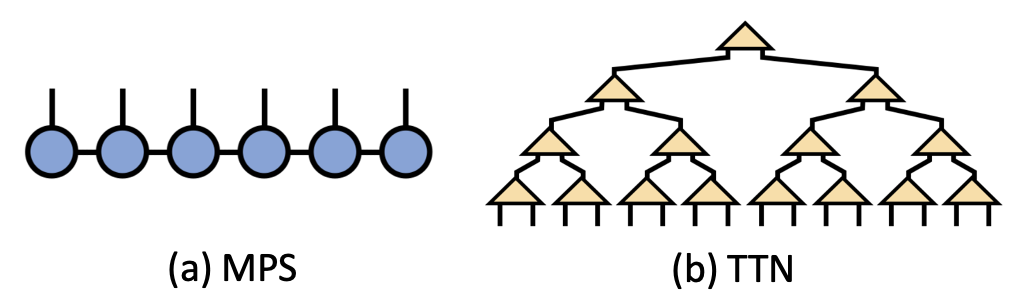
\includegraphics[width=\columnwidth]{groups/3._Classical_simulation_of_quantum_systems/MPS-TTN.png}
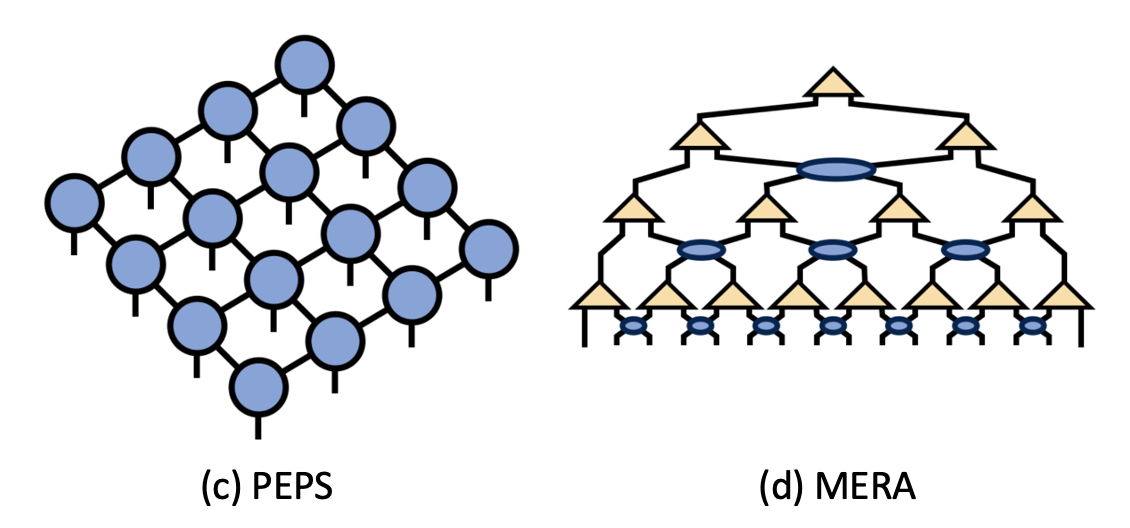
\includegraphics[width=\columnwidth]{groups/3._Classical_simulation_of_quantum_systems/PEPS-MERA.png}
\caption{Different types of tensor network simulators: (a) Matrix Product States (MPS), (b) Tree Tensor Networks (TTN), (c) Projected Entangled Pair States (PEPS), and (d) Multi-scale Entanglement Renormalization Ansatz (MERA).}
\label{fig:tensornetworks}
\end{figure}

Each type of tensor network has its specific applications, advantages, and limitations, and the choice of which to use depends on the application, size, and structure of a quantum circuit:
\begin{itemize}
    
\item MPS simulators excel in one-dimensional quantum systems with short-range interactions. They are efficient for simulating ground and excited states, as well as dynamical properties, due to their ability to capture entanglement in a scalable manner with limited entanglement entropy.

\item  PEPS are generalizations of MPS to higher dimensions, making them suitable for two-dimensional quantum systems. They are adept at handling both short- and long-range interactions, but their computational complexity increases significantly with the system's size and entanglement.

\item  TTN simulators are structured in a hierarchical, tree-like manner, offering efficient computation for certain quantum circuits, especially those with hierarchical or layered structures. They are particularly useful for simulating states that exhibit hierarchical entanglement patterns and for providing insights into quantum many-body systems.

\item  MERA is designed for critical systems with long-range entanglement. It excels in representing ground states of quantum many-body systems near criticality, offering insights into scaling and universality in quantum phase transitions.

\item  CTVN simulators are tailored for quantum systems with continuous variables, like quantum fields or modes of light. They are adept at handling systems where particle number isn't conserved and are crucial in studying non-Gaussian states and processes in quantum optics and field theories.
\end{itemize}

Tensor network simulators continue to evolve, with ongoing research aimed at increasing their efficiency, scalability, and applicability to a broader range of quantum computing tasks.


\subsubsection{Open system Lindblad quantum simulators}

Open-system Lindblad quantum simulators are specifically designed to model the dynamics of quantum systems interacting with external environments. The applications include, for example, simulating quantum magnetism, topological materials, 
quantum phase transitions, and electron transportation. Unlike closed quantum systems, open systems are subject to environmental influences that lead to non-unitary processes such as decoherence and dissipation. These simulators leverage the Lindblad master equation, which blends the unitary evolution dictated by the system's Hamiltonian with the non-unitary aspects resulting from environmental interactions. This approach allows for a comprehensive simulation of open quantum systems, capturing the complexity of quantum noise and the environmental effects. Recently, a novel approach, called noisy quantum gates, has been proposed, as a classical simulation of the Lindblad dynamics~\cite{noisygates}. It is based on integrating the noise into the gates, rather than keeping gates and noise as two separate dynamics, an approach can be generalized to non-Markovian dynamics by using colored noises.

In general, there are a few ways to formulate, but the most common is to use the density matrix formalism, which is adept at representing mixed states, a critical aspect when dealing with open systems. These simulators provide researchers with the flexibility to define specific system-environment interactions, making them a versatile tool across various quantum research domains, especially in material science applications. Its ability to accurately model quantum noise induced by the environment is an especially valuable aspect of it. Overall, the open-system Lindblad quantum simulators stand as a very valuable tool in quantum research, enabling a deeper understanding of the environmental impacts on quantum systems and aiding in the advancement of practical quantum applications.


\subsection{Overview of classical simulators}

In summary, we described four main types of quantum circuit simulators. In the context of material science, the choice of a quantum circuit simulator depends on the specific characteristics of the system under study and the phenomena of interest. Here is how each type of simulator can be used:

State-vector simulators are ideal for systems that can be accurately represented by pure quantum states. In material science, they are particularly useful for studying the evolution of quantum states under Hamiltonians with relatively few degrees of freedom. They excel in scenarios where the full quantum state needs to be tracked, such as in the simulation of small, isolated quantum systems or systems with limited entanglement.

Density matrix simulators are well suited for studying systems where mixed states are prevalent, which includes most real-world scenarios in material science. They can handle decoherence and other noise effects, making them suitable for simulating open quantum systems or systems under non-ideal conditions. Density matrix simulators are ideal for investigating phenomena in quantum materials where environmental interactions play a significant role.

Different types of tensor network simulators have different use cases.
MPS and TTN are powerful in simulating one-dimensional and certain hierarchical quantum systems, respectively. They can efficiently model systems with short-range interactions, which are common in material science. These simulators are especially useful for studying ground state properties and low-energy excitations in materials.
PEPS and MERA are more suited for higher-dimensional systems. PEPS can handle both short- and long-range interactions in two-dimensional materials, making them valuable for exploring complex quantum materials, such as high-temperature superconductors. MERA is particularly effective in studying critical phenomena and phase transitions in materials.

Open system Lindblad quantum simulators are designed to handle non-unitary evolution, which is typical in open quantum systems, where the system is in contact with an external environment. In material science, they are crucial for studying decoherence, dissipation, and thermalization processes in materials. Lindblad simulators are particularly relevant for investigating quantum materials and devices operating under realistic, non-ideal conditions, where environmental interactions cannot be ignored. They are essential for understanding the behavior of materials in quantum information processing and quantum sensing applications, where control and mitigation of decoherence are critical.

Using HPC is critical for simulating large quantum circuits. Ultimately, supercomputers can simulate relatively small quantum circuits because of the exponential requirement of available distributed memory. The next generation of quantum simulators will probably use small quantum computers to simulate very large quantum circuits. The idea is to use small quantum computers to perform tasks that are inherently quantum in nature, such as the contraction of intermediate multi-dimensional tensors, which are central to tensor network simulations. This idea is closely related to Feynman's proposal to use quantum computers to simulate quantum systems~\cite{hey2018feynman}. One way is to use Harrow-Hassidim-Lloyd (HHL) algorithm for the contraction of very high-dimension tensors, which is currently a bottleneck of classical tensor network simulators. The HHL algorithm can be adapted to perform tensor contractions by encoding the tensors as linear systems. This could potentially revolutionize tensor network simulations by dramatically reducing the computational complexity of these contractions. This approach promises a scalable pathway for quantum simulation, as improvements in quantum hardware, such as increased qubit counts and enhanced coherence times, would directly translate into an increased capacity for simulating larger and more complex quantum circuits.

\iffalse
\subsection{Simulation of time dynamics} 
Move to another section.

People: Yuri Alexeev, Burns Healy, Bo Phang, Niri Govind

Describe here the challenges of simulating time dynamics classically and make the case for quantum simulations. Cover topics such as simulation of quantum effects, scalability, and accuracy.

Write text on Yang-Baxter circuit compression. Describe how to perform these calculations efficiently and the challenges for achieving quantum advantage.

The time evolution of quantum systems described by Ising-type Hamiltonians is a very important problem in condensed matter physics and quantum information. These Hamiltonians encompass a wide range of physical phenomena, from magnetic interactions in condensed matter systems to the formulation of optimization problems for quantum computing. In particular, the Ising model describes a lattice of spins with pairwise interactions, characterized by a Hamiltonian that depends on the arrangement of spins and the interaction strengths between them. The general form of an Ising-type Hamiltonian is given by:

\begin{equation}
H = -\sum_{i, j} J_{ij}(t) \sigma_i \sigma_j - \sum_{i} h_i(t) \sigma_i,
\label{ising_hamiltonian}
\end{equation}

where $\sigma_i^z$ and $\sigma_i^x$ represent Pauli matrices, $J_{ij}(t)$ are time-dependent coupling strengths, $h_i(t)$ are time-dependent magnetic fields, and the summations extend over all pairs of spins and single-spin terms.

The problem of accurate large-scale time dynamics simulations remains an area of active research. List the challenges (noise, size, time dynamics length) and opportunities.


\subsection{Simulation of ground states}

Quantum Monte Carlo, etc. 

\subsection{Simulation of finite-temperature systems}

\fi









\section{Classical simulation of quantum systems\label{sec:ClassicalSimulationOfQSystems}}

\subsection{Why use classical simulators}

For near-term quantum computers, one might question the necessity of classical simulators to emulate quantum computations. After all, the promise of quantum computing lies in its ability to perform certain tasks exponentially faster than classical computers. However, classical simulators remain invaluable for several compelling reasons \cite{10.1038/s41598-019-47174-9, 9910084,doi.org/10.48550,Fedorov2022unitaryselective,preopt-0,preopt-1,preopt-2,IBMQuantumSummit2023}.

\begin{enumerate}
    \item {\bf Resource Efficiency:} Quantum computer time is a limited and valuable resource. When developing and testing new quantum circuits or algorithms, researchers often need to execute them numerous times to validate their functionality and robustness. Running experiments on a real quantum machine can be time-consuming and costly, particularly when waiting for quantum computer availability after each circuit modification. Classical simulators offer an efficient alternative, allowing researchers to rapidly iterate through experiments without waiting for quantum resources.
    \item {\bf Noise and Error Analysis:} Real quantum machines are susceptible to noise and errors due to environmental factors, making it challenging to control and maintain the desired quantum state fidelity. Classical simulators provide a controlled environment for introducing and analyzing various noise scenarios. Researchers can simulate quantum noises to assess how robust their algorithms are under different conditions, as well as explore error correction techniques. This is a crucial step in building fault-tolerant quantum systems.
    \item {\bf Scalability:} Current quantum machines have limitations in terms of the number of qubits and the noise levels they exhibit. Classical simulators, on the other hand, can be adapted to simulate quantum systems with a larger number of qubits, enabling researchers to explore complex quantum algorithms and states that are beyond the capabilities of existing quantum hardware.
    \item {\bf Versatility:} Classical simulators offer flexibility regarding what they can simulate. Researchers can use them to capture "snapshots" of quantum states during computations, perform measurements, and make decisions based on measurement outcomes. Additionally, they can obtain more comprehensive information, such as the density operator of the system, rather than just specific measurement results.
    \item {\bf Efficiency Trade-Offs:} Building an efficient quantum simulator involves addressing trade-offs between computational efficiency and the range of quantum states it can represent. The choice of simulator depends on the specific needs of the quantum computation being emulated.
    \item {\bf Connectivity:}
    When executing a circuit on quantum hardware, the transpilation step involves mapping logical qubits to physical ones, in a fashion that may one-to-many. This is due to the constraint of the physical connection of qubits, which is not usually all-to-all on true QPUs. When simulating, all qubits can be entangled with all others, thus keeping down the `physical' qubits needed and easing the computational burden of solving the minor-embedding problem.
  \item {\bf Pre-optimization:}
    Variational algorithms can be expensive and require many iterations of a quantum circuit.  Pre-optimization with classical simulators can be used to find approximate circuits parameters that can be used or refined with quantum hardware.\cite{preopt-0,preopt-1,preopt-2}
    \item {\bf HPC-assisted quantum computing:}
    There is a way in which HPC can substantially help to extend the depth of quantum circuits, as demonstrated in the recently developed method called "Operator Backpropagation."~\cite{IBMQuantumSummit2023} The idea is to compute a part of a quantum circuit on a quantum device, and compute the second part of a circuit classically by using a quantum circuit simulator on an HPC system, and then stitch the results together. 
\end{enumerate}
In summary, classical simulators allow for efficient development, testing, and analysis of quantum circuits, algorithms, and states, while also providing a controlled environment for exploring quantum noise and errors. While quantum computers hold immense promise, classical simulators remain a vital component of the quantum computing toolkit, enabling progress and innovation in the field. Furthermore, simulators will likely continue to serve as yet another type of circuit execution environment among multi-node compute clusters for executing distributed workloads, which will be adept at handling (sub-)circuits that fall within their scope.

\subsection{Quantum circuits simulators}

In this section, we describe different types of classical quantum circuit simulators. In particular, we describe their capabilities in terms of what the maximum size systems (in both qubits and gates) that can be simulated using HPC. The advantages and disadvantages of quantum circuit simulators are also discussed, as well as use cases.

Before we start, we note that not every quantum circuit is difficult to simulate on a classical computer. Trivially, a quantum circuit that carries out a purely classical computation is not difficult to simulate on a classical computer. Indeed, some of the quantum circuits that are not difficult to simulate include Clifford circuits~\cite{gottesman1998heisenberg,aaronson2004improved,garcia2014simulation} and the quantum Fourier transform~\cite{aharonov2006quantum,yoran2007efficient}, to name a couple. Some quantum circuits are known to be classically simulable for specific input states as well~\cite{garcia2014simulation}. If the simulation does not need to produce the full spectrum of the output state of a given quantum computation but rather a sampling of such, as it would be the case for obtaining a final, classical result out of a quantum computer upon measurements, the difficulty of the classical simulation can dramatically decrease~\cite{hillmich2020just}. Further decrease in the difficulty is obtained if the simulation is to mimic an error-prone quantum computer executing a quantum circuit~\cite{hillmich2022approximating}. We further note in passing that simulation of a quantum circuit that exhibits sparse couplings between densely connected sets of qubits can be more amenable to classical simulations~\cite{fatima2021faster}, using methodologies not unlike circuit cutting discussed in Sec.~\ref{sec:CNA}.

\subsubsection{State-vector simulators}

State-vector based simulation is to simulate the operations of applying a series of unitary operators $U_{m-1} \cdots U_1 U_0$ to the state-vector representation of the quantum states $\ket{\psi}=\sum_{i=0}^{2^n-1}\alpha_i\ket{i}$, where $n$ is the number of qubits and $m$ is the number of operations or gates. Typically, a complex-valued double or single precision floating-point vector $\vec{\alpha}$ of size $2^n$ is used to store the coefficients $\alpha_i$, which costs $16\times2^n$ bytes of memory for classical simulation. $U_i$ with $i\in[0,m-1]$ is a $2\times2$ (for one-qubit gate) or $4\times4$ (for two-qubit gate) complex matrix. It has been shown that an arbitrary quantum circuit can be decomposed into 1-qubit and 2-qubit gates \cite{barenco1995elementary}. In fact, most quantum devices internally run 1-qubit or 2-qubit basis gates. For example, IBM adopts 1-qubit gate \texttt{X}, \texttt{SX}, \texttt{RZ}, \texttt{ID} and 2-qubit gate \texttt{CX} (recently \texttt{ECR}) as the basis gates. To apply a gate $U$, the operation is $\ket{\psi}\to U\ket{\psi}$. For 1-qubit $U$ applying on qubit $q$ in a quantum register, $\vec{\alpha}$ is updated through the following expression where $s_i=\lfloor i/{2^q}\rfloor 2^{q+1}+(i \% 2^q)$ for every integer $i\in[0, 2^{n-1}-1]$:
\begin{equation}
\begin{bmatrix}
\alpha_{s_i} \\
\alpha_{s_i+2^q}  
\end{bmatrix}
\to
U_{2\times2}\cdot \begin{bmatrix}
\alpha_{s_i} \\
\alpha_{s_i+2^q}  
\end{bmatrix}
\label{eq:1q-op}
\end{equation}
Regarding 2-qubit unitary gate $U$ applying on qubit $p$ and $q$ (assuming $p<q$ without losing generality), $\vec{\alpha}$ is updated  through:
\begin{equation}
\begin{bmatrix}
\alpha_{s_i} \\
\alpha_{s_i+2^p} \\
\alpha_{s_i+2^q} \\
\alpha_{s_i+2^p+2^q}
\end{bmatrix}
\to
U_{4\times4}\cdot \begin{bmatrix}
\alpha_{s_i} \\
\alpha_{s_i+2^p} \\
\alpha_{s_i+2^q} \\
\alpha_{s_i+2^p+2^q}
\end{bmatrix}
\label{eq:2q-op}
\end{equation}
where $s_i{=}\lfloor \lfloor i/{2^p}\rfloor /2^{q-p-1} \rfloor  2^{q+1} + (\lfloor i/{2^p}\rfloor \% 2^{q-p-1})2^{p+1} +  (i \% 2^p)$ for every integer $i\in[0,2^{n-2}-1]$. 

Therefore, state-vector based quantum numerical simulation is to perform a sequence of $2\times2$ or $4\times4$ operations Eq.~(\ref{eq:1q-op}) and Eq.~(\ref{eq:2q-op}) over the large state-vector coefficient array of complex numbers in a classical system.

State vector simulators hold the full coefficients of pure quantum states within the classical system's memory, which scales exponentially with the number of qubits. Consequently, the state vector is often distributed across many nodes of a classical HPC~\cite{haner20170,pednault2017breaking,pednault2019leveraging,li2021sv}. Such simulators however exhibit linear scaling with respect to the circuit depth~\cite{fatima2021faster}. As such, state vector simulations are sensitive to the number of qubits but much less to the gate count or circuit depth. For example, a recent work shows that a low-energy nuclear quantum circuit with 115 million gates on 21-qubits can be effectively simulated within one hour using a GPU for state vector simulation~\cite{li2023deep}.

We note that various forms of approximate state-vector simulators can be tailored to problem specific applications.  For example, recent truncated state vector simulators have been used to simulate VQE for various chemistry problems on 64 qubits without significant loss of accuracy or the need for large computing resources~\cite{preopt-2,approxstatevec}. Combining the state vector simulators with Feynman path summation can trade the circuit depth with the number of qubits or memory usage~\cite{fatima2021faster}, rendering some hard to simulate circuits according to a naive state vector simulator to be simulable due to orders of magnitude improvement in their simulability~\cite{markov2020massively,fatima2021faster}.

\subsubsection{Density matrix simulators}

When dealing with a mixed system where noise is present, a pure state can no longer provide sufficient information about the system. In this case, a mixed state corresponds to a statistical ensemble, or probabilistic mixture of pure states, can be used to describe the condition where a system is entangled with another system, such as the environment from which the noise is imposed. A mixed state is represented by a density matrix or a density operator, which is defined by choosing the basis in the underlying space. The density matrix is given by:
\begin{equation*}
\rho=\sum{p_s\ket{\psi_s}\bra{\psi_s}}
\end{equation*}
where $\rho$ represents the fraction of the ensemble of each pure state and is generally an unknown real value. A density matrix contains all the information of a quantum system, allowing the calculation of the probabilities of the outcomes of any measurement performed.

Compared to state-vector simulation, the density operator requires the conservation of $4^n$ coefficients, where $n$ is the number of eigenstates for each pure state, i.e., the number of qubits. Therefore, the memory cost of a density matrix simulation is $2^n$ times that of a pure state simulation using state-vector. The system also evolves according to the operator or gate sequence. When a particular gate is applied, the density matrix evolves as follows~\cite{li2020density}:
\begin{equation}
\rho(t)=G(t)\rho(0)G(t)^{\dagger}
 \label{eq:onegate}
\end{equation}
where $G(t)$ is the gate at time $t$, and $G(t)^\dagger$ is its adjoint. The evolution of a density matrix is more complicated than that of a state vector, considering the size of $4^n$ and the extra adjoint operator per gate. Although $G(t)$ by itself is a unitary operator, it becomes a general matrix and is not necessarily unitary in the presence of noise. Depending on the noise model, the evolution can become an ensemble of evolutions of corresponding channels, each described by a Kraus operator.

The noisy density matrix quantum numerical simulation is to compute $\rho_\text{out}$ for a n-qubit quantum system, density matrix quantum circuit simulation is to compute $\rho_\text{out}$ for a n-qubit quantum register, given initial state $\rho_\text{in}$ and $m$ non-unitary transformations $G_0$, $G_1$, $\dots$, $G_{m-1}$:
\begin{equation}
 \rho_{\text{out}} = G_{m-1}\cdots (G_1 (G_0 \rho_{\text{in}} G^\dag_0) G^\dag_1)\cdots G^\dag_{m-1}
 \label{eq:dmsim}
\end{equation}
where $G$ and $\rho$ are $2^n\times 2^n$ matrices. Due to noise, $G$ is not necessarily a unitary matrix. $G^\dag$ is the adjoint of $G$ verifying $G^\dag=(G^*)^T$. As real quantum devices typically use 1-qubit or 2-qubit gates representing as $4\times4$ or $16\times16$ matrices, to obtain the matrix $G_i$ with a $2^n\times2^n$ size, Kronecker product or tensor product is used with the identity matrix $I$ for the other qubits. 


\subsubsection{Tensor network simulators}

Quantum tensor networks can be used for the simulation of quantum circuits~\cite{markov2008simulating, lykov2021importance, lykov2021large, lykov2021performance, lykov2022tensor, berquist2022stochastic, shah2023gpu}. These simulators leverage the mathematical framework of tensor networks, which are graphical representations of quantum states and operations, as networks of interconnected tensors. Specifially, the nodes in these networks correspond to tensors, which encode gate operations, while the edges represent indices along which tensors are contracted, reflecting the entanglement and interactions between qubits.

The strength of tensor network simulators lies in their ability to compactly represent quantum states that would otherwise require a prohibitive amount of memory. This is particularly valuable for simulating shallow-depth quantum circuits with a large number of qubits, which are challenging for traditional state-vector simulators. These simulators are still limited by the amount of available distributed memory on a supercomputer. For the current generation of supercomputers, tensor network simulators can run quantum circuits up to approximately 200 qubits without approximations for certain quantum circuits~\cite{lykov2021large}. Larger simulations are possible with a truncated bond dimension as well as other applications with different resource requirements~\cite{preopt-1}.


There are different types of tensor network simulators: Matrix Product States (MPS), Projected Entangled Pair States (PEPS), Tree Tensor Networks (TTN), Multi-scale Entanglement Renormalization Ansatz (MERA), and Continuous Variable Tensor Network (CVTN) to name a few as shown on Figure~\ref{fig:tensornetworks}. MPS is arguably one of the most popular simulators, and it is particularly useful for simulating one-dimensional quantum systems. In MPS, the tensors are arranged in a chain, with each tensor representing the state of a qubit and the connections between them capturing the nearest-neighbor entanglement. One of the MPS applications is an efficient tensor network simulation of lossy Gaussian boson sampling experiments, which has been recently demonstrated \cite{liu2023simulating, Oh2023}.
%{\color{red}Minh: Can we briefly comment on when the other methods (PEPS, TTN, ...) are good?}

\begin{figure}
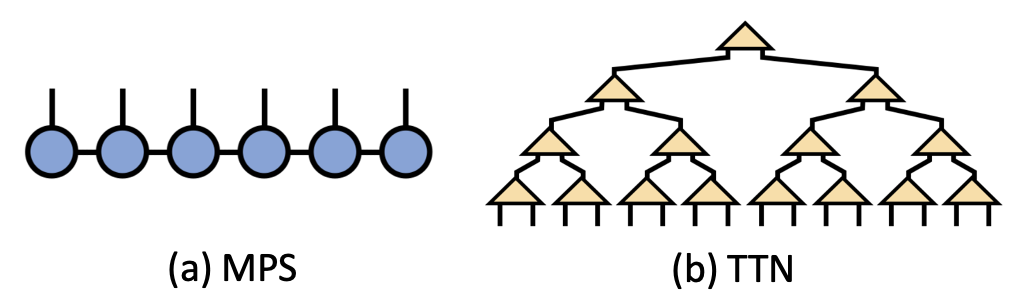
\includegraphics[width=\columnwidth]{groups/3._Classical_simulation_of_quantum_systems/MPS-TTN.png}
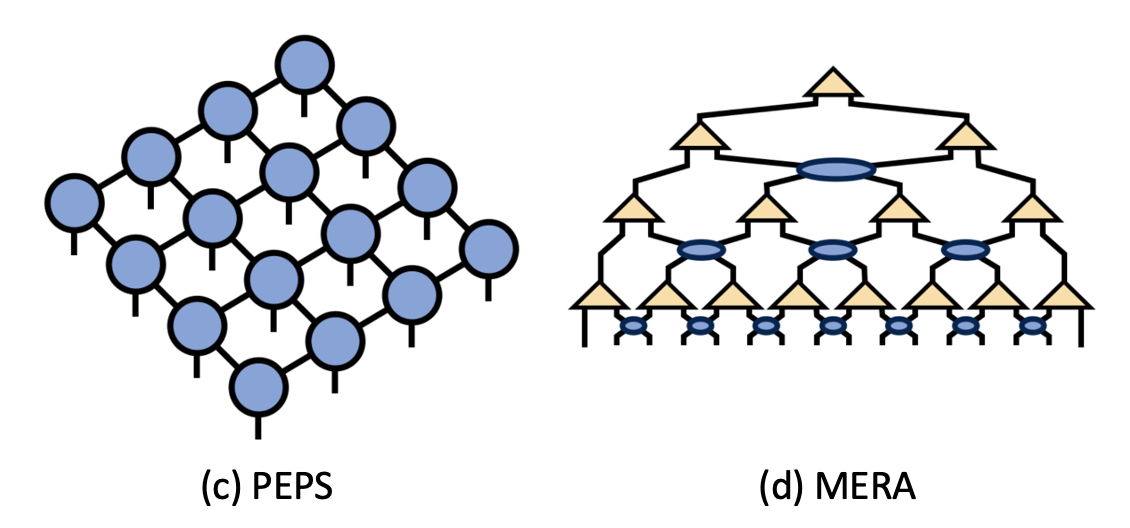
\includegraphics[width=\columnwidth]{groups/3._Classical_simulation_of_quantum_systems/PEPS-MERA.png}
\caption{Different types of tensor network simulators: (a) Matrix Product States (MPS), (b) Tree Tensor Networks (TTN), (c) Projected Entangled Pair States (PEPS), and (d) Multi-scale Entanglement Renormalization Ansatz (MERA).}
\label{fig:tensornetworks}
\end{figure}

Each type of tensor network has its specific applications, advantages, and limitations, and the choice of which to use depends on the application, size, and structure of a quantum circuit:
\begin{itemize}
    
\item MPS simulators excel in one-dimensional quantum systems with short-range interactions. They are efficient for simulating ground and excited states, as well as dynamical properties, due to their ability to capture entanglement in a scalable manner with limited entanglement entropy.

\item  PEPS are generalizations of MPS to higher dimensions, making them suitable for two-dimensional quantum systems. They are adept at handling both short- and long-range interactions, but their computational complexity increases significantly with the system's size and entanglement.

\item  TTN simulators are structured in a hierarchical, tree-like manner, offering efficient computation for certain quantum circuits, especially those with hierarchical or layered structures. They are particularly useful for simulating states that exhibit hierarchical entanglement patterns and for providing insights into quantum many-body systems.

\item  MERA is designed for critical systems with long-range entanglement. It excels in representing ground states of quantum many-body systems near criticality, offering insights into scaling and universality in quantum phase transitions.

\item  CTVN simulators are tailored for quantum systems with continuous variables, like quantum fields or modes of light. They are adept at handling systems where particle number isn't conserved and are crucial in studying non-Gaussian states and processes in quantum optics and field theories.
\end{itemize}

Tensor network simulators continue to evolve, with ongoing research aimed at increasing their efficiency, scalability, and applicability to a broader range of quantum computing tasks.


\subsubsection{Open system Lindblad quantum simulators}

Open-system Lindblad quantum simulators are specifically designed to model the dynamics of quantum systems interacting with external environments. The applications include, for example, simulating quantum magnetism, topological materials, 
quantum phase transitions, and electron transportation. Unlike closed quantum systems, open systems are subject to environmental influences that lead to non-unitary processes such as decoherence and dissipation. These simulators leverage the Lindblad master equation, which blends the unitary evolution dictated by the system's Hamiltonian with the non-unitary aspects resulting from environmental interactions. This approach allows for a comprehensive simulation of open quantum systems, capturing the complexity of quantum noise and the environmental effects. Recently, a novel approach, called noisy quantum gates, has been proposed, as a classical simulation of the Lindblad dynamics~\cite{noisygates}. It is based on integrating the noise into the gates, rather than keeping gates and noise as two separate dynamics, an approach can be generalized to non-Markovian dynamics by using colored noises.

In general, there are a few ways to formulate, but the most common is to use the density matrix formalism, which is adept at representing mixed states, a critical aspect when dealing with open systems. These simulators provide researchers with the flexibility to define specific system-environment interactions, making them a versatile tool across various quantum research domains, especially in material science applications. Its ability to accurately model quantum noise induced by the environment is an especially valuable aspect of it. Overall, the open-system Lindblad quantum simulators stand as a very valuable tool in quantum research, enabling a deeper understanding of the environmental impacts on quantum systems and aiding in the advancement of practical quantum applications.


\subsection{Overview of classical simulators}

In summary, we described four main types of quantum circuit simulators. In the context of material science, the choice of a quantum circuit simulator depends on the specific characteristics of the system under study and the phenomena of interest. Here is how each type of simulator can be used:

State-vector simulators are ideal for systems that can be accurately represented by pure quantum states. In material science, they are particularly useful for studying the evolution of quantum states under Hamiltonians with relatively few degrees of freedom. They excel in scenarios where the full quantum state needs to be tracked, such as in the simulation of small, isolated quantum systems or systems with limited entanglement.

Density matrix simulators are well suited for studying systems where mixed states are prevalent, which includes most real-world scenarios in material science. They can handle decoherence and other noise effects, making them suitable for simulating open quantum systems or systems under non-ideal conditions. Density matrix simulators are ideal for investigating phenomena in quantum materials where environmental interactions play a significant role.

Different types of tensor network simulators have different use cases.
MPS and TTN are powerful in simulating one-dimensional and certain hierarchical quantum systems, respectively. They can efficiently model systems with short-range interactions, which are common in material science. These simulators are especially useful for studying ground state properties and low-energy excitations in materials.
PEPS and MERA are more suited for higher-dimensional systems. PEPS can handle both short- and long-range interactions in two-dimensional materials, making them valuable for exploring complex quantum materials, such as high-temperature superconductors. MERA is particularly effective in studying critical phenomena and phase transitions in materials.

Open system Lindblad quantum simulators are designed to handle non-unitary evolution, which is typical in open quantum systems, where the system is in contact with an external environment. In material science, they are crucial for studying decoherence, dissipation, and thermalization processes in materials. Lindblad simulators are particularly relevant for investigating quantum materials and devices operating under realistic, non-ideal conditions, where environmental interactions cannot be ignored. They are essential for understanding the behavior of materials in quantum information processing and quantum sensing applications, where control and mitigation of decoherence are critical.

Using HPC is critical for simulating large quantum circuits. Ultimately, supercomputers can simulate relatively small quantum circuits because of the exponential requirement of available distributed memory. The next generation of quantum simulators will probably use small quantum computers to simulate very large quantum circuits. The idea is to use small quantum computers to perform tasks that are inherently quantum in nature, such as the contraction of intermediate multi-dimensional tensors, which are central to tensor network simulations. This idea is closely related to Feynman's proposal to use quantum computers to simulate quantum systems~\cite{hey2018feynman}. One way is to use Harrow-Hassidim-Lloyd (HHL) algorithm for the contraction of very high-dimension tensors, which is currently a bottleneck of classical tensor network simulators. The HHL algorithm can be adapted to perform tensor contractions by encoding the tensors as linear systems. This could potentially revolutionize tensor network simulations by dramatically reducing the computational complexity of these contractions. This approach promises a scalable pathway for quantum simulation, as improvements in quantum hardware, such as increased qubit counts and enhanced coherence times, would directly translate into an increased capacity for simulating larger and more complex quantum circuits.

\iffalse
\subsection{Simulation of time dynamics} 
Move to another section.

People: Yuri Alexeev, Burns Healy, Bo Phang, Niri Govind

Describe here the challenges of simulating time dynamics classically and make the case for quantum simulations. Cover topics such as simulation of quantum effects, scalability, and accuracy.

Write text on Yang-Baxter circuit compression. Describe how to perform these calculations efficiently and the challenges for achieving quantum advantage.

The time evolution of quantum systems described by Ising-type Hamiltonians is a very important problem in condensed matter physics and quantum information. These Hamiltonians encompass a wide range of physical phenomena, from magnetic interactions in condensed matter systems to the formulation of optimization problems for quantum computing. In particular, the Ising model describes a lattice of spins with pairwise interactions, characterized by a Hamiltonian that depends on the arrangement of spins and the interaction strengths between them. The general form of an Ising-type Hamiltonian is given by:

\begin{equation}
H = -\sum_{i, j} J_{ij}(t) \sigma_i \sigma_j - \sum_{i} h_i(t) \sigma_i,
\label{ising_hamiltonian}
\end{equation}

where $\sigma_i^z$ and $\sigma_i^x$ represent Pauli matrices, $J_{ij}(t)$ are time-dependent coupling strengths, $h_i(t)$ are time-dependent magnetic fields, and the summations extend over all pairs of spins and single-spin terms.

The problem of accurate large-scale time dynamics simulations remains an area of active research. List the challenges (noise, size, time dynamics length) and opportunities.


\subsection{Simulation of ground states}

Quantum Monte Carlo, etc. 

\subsection{Simulation of finite-temperature systems}

\fi












\section{Conclusions and Outlook\label{sec:conclusion_outlook}}

In this paper we have described applications from experimental and theoretical high-energy physics where quantum computing has the potential to show a better performance than their classical counterparts. The selected applications were chosen also with respect to IBM's 100$\otimes$100 challenge and, where possible, a resource estimate was made. We note that the given applications are by no means complete and should serve as examples which are of very high interest for the high-energy physics community. We emphasize that this work should serve as an initial step by the present authors for exploring the potential of quantum computing for high-energy physics and we expect that the community of high-energy physicists working on this will substantially grow in the future. 

Concerning the quantum algorithms proposed for the applications outlined in the theory section (\ref{subsect_Theory}), we have identified quantum dynamics as one of the main targets because of its relevance in the field of \gls{hep}, e.g., in scattering phenomena, string breaking, quenching or dynamical properties of phase transitions. 
In fact, the exponentially growing costs of the corresponding classical approaches combined with  
the availability of well-tuned quantum algorithms make quantum computing a very promising tool for tackling problems in quantum dynamics. 
As already outlined in the theory section in table~\ref{table:resources}, such quantum dynamics applications are indeed compatible 
with the $100 \otimes 100$ challenge. 
Besides the dynamical aspects of theoretical \gls{hep} models applications we have also described static situations where quantum computing could lead to a better performance. These include abelian and non-abelian lattice gauge theories supplied with topological terms or non-zero fermion density or investigations of neutrino oscillations. While for these cases quantum computing has clearly an advantage over classical Markov Chain Monte Carlo methods it remains to be seen, whether it will have advantages over tensor network approaches, e.g. when taking the continuum limit or close to a phase transition. 

In this paper, we have identified and proposed concrete examples of low (1+1)D and (2+1)D theoretical models of \gls{hep} (and in particular lattice gauge theory) which are particularly hard classically due to the level of the entanglement produced, but still preserve a great physical relevance as prototypes for understanding fundamental dynamic but also static aspects of the laws of Nature.  
In the path towards large-scale simulations, we propose the development of hybrid quantum-classical algorithms, which can optimally leverage the advantages offered by the two complementary computational paradigms; for instance, the combination of \gls{tn} with quantum circuit representation of the system wave function can offer a unique opportunity for enabling the simulations of strongly entangled systems for longer time scales or close to phase transitions.

We consider the here proposed models as an intermediate step towards eventually reaching (3+1)D theories as actually needed  for studying the standard model of \gls{hep}. Besides the fact that the here considered lower dimensional models are of a high interest by themselves, we are convinced that investigating them with quantum computing can significantly help to develop algorithms and methods for studying their (3+1)D counterparts. And, it is a really fascinating outlook to explore phases of \gls{qcd} where no one has looked before such as the very eaerly universe or when the strenghts of a topological term becomes large. In addition, it would allow to study scattering phenomena in a fully non-perturbative fashion opening completely new insight to the physics of article collisons and shed light on the transition of confined phase of \gls{qcd} to the quark gluon plasma. 

A wide variety of \gls{qc} applications are anticipated in quantum simulations and \gls{hep} experimental workflow, as described in the earlier sections. Quantum simulations of simplified \gls{lgt}s in the Standard Model, such as \gls{2p1D} \gls{qed} or \gls{2p1D} SU(2) theory, are potential, well-motivated applications for near-term quantum computers. For the experimental side, \gls{qml} is a major technique to exploit quantum computing in the applications such as signal processing and detector reconstruction. 
However, as mentioned in Section~\ref{subsect_Experiments}, when considering \gls{qml} for processing classical experimental data, the data encoding into a quantum circuit is a big challenge, in particular for future colliders where an enormous amount of data will be produced. Moreover, the data encoding is also known to be one of the critical processes that cause barren plateau. 

This motivates us to explore the possibility of utilizing {\it quantum data} in the future as a promising route to directly exploit quantum properties encoded in quantum simulation and \gls{hep} experimental data.
From a theoretical perspective, understanding the power of quantum data for learning quantum states has received a lot of attention. There has been a sequence of works in tomography, wherein a learner is given copies to an unknown $n$-qubit quantum state $\rho$ and needs to learn $\rho$ well-enough (up to $\varepsilon$-trace distance); here the sample complexity was pinned down~\cite{haah2017sample,o2016efficient} to $\Theta(2^{2n}/\varepsilon^2)$. 
However, the exponential nature of learning an unknown quantum state is undesirable; there have been works that have looked at restricted classes of states and shown that they are learnable using polynomially many copies of the states, such as stabilizer states~\cite{montanaro2017learning}, Gibbs states of local Hamiltonians~\cite{anshu2021sample}, matrix product states~\cite{CPFSGBLPL10}. Another body of work has considered the setting in which the goal is not to learn the entire unknown quantum state $\rho$ but to learn only certain properties of $\rho$. In this context, people have considered tasks such as $(i)$ PAC learning: the learning algorithm here is given access to $(E_i,\Tr(\rho E_i))$ where  $\{E_i,\mathbb{I}-E_i\}$ is a uniformly random \gls{povm} element, $(ii)$ Shadow tomography, where the goal is, given copies of an unknown quantum state $\rho$, can we learn the expectation values of $\rho$ with respect to a certain set of \emph{fixed, a priori known} observables $\{E_1,\ldots,E_m\}$, $(iii)$ Other models such as classical shadows, online learning, learning with differential privacy that have modified the models $(i,ii)$. In all these models of learning, it is well-established  that~\cite{aaronson:shadow,aaronson2018online,aaronson2007learnability} the complexity of learning is $\mathcal{O}(n)$, which is \emph{exponentially} better than tomography.  For a detailed survey on the complexity of learning quantum data, we refer the interested reader to~\cite{anshusurvey}.

More practical applications of quantum data learning to \gls{hep} is to use it for extracting physical information from quantum states in quantum simulation.
This was first proposed in the context of condensed-matter physics~\cite{2019NatPh..15.1273C}
and further explored in~\cite{2021arXiv210612627H,2021PRXQ....2d0321B,PhysRevA.102.012415,2021arXiv210903400S,bernien2017probing, 2021arXiv210306712B,monaco2023quantum}.
The typical example is a recognition of quantum phases, where the \gls{qml} model learns the pair of quantum states and their phases to predict phase of unknown states.
In the context of high-energy physics, we often encounter phase transitions that cannot be investigated by local order parameters, such as confinement/deconfinement transition in \gls{qcd}.
It would be interesting to apply quantum data learning method to extract physical information in such situations.


In the longer-term, one may perform quantum experiment, not only digital quantum simulation but also analogue quantum simulation or others, then measure the final states via quantum sensor, and transduce the states coherently to a quantum computer which performs \gls{qml} to extract physical information~(see e.g., \cite{Huang_2022}).
This hybrid system could be extended to the concept of quantum-enhanced \gls{hep} experiment. A fascinating direction to exploit quantum data is to physically place quantum sensing devices in experiments and directly feed quantum states registered on the sensors into quantum computers. This certainly involves many challenges, e.g., detect particles or wave-like matters in quantum sensor, coherently transfer the generated state to other quantum systems, perform quantum operations to measure physical properties within coherence time. Such experiments will, however, provide an exciting opportunity to directly explore quantum phenomena observed in \gls{hep} experiments and extract dynamical properties of entangled quantum states.

A `\textit{conditio sine qua non}' for the success of this program in the era of noisy, near-term quantum devices is the co-design of error mitigation schemes that can efficiently compensate for  the different noise sources (e.g., gate errors, qubit decoherence and cross-talk) and guarantee results of sufficient quality to extract the physics of interest. To this end, several error mitigation schemes have been proposed in the past few years (see Sec.~\ref{sec:ibm_roadmap}) including zero-noise extrapolation~\cite{Temme2017Error}, probabilistic error cancellation~\cite{Berg2022Probabilistic}, and the probabilistic error amplification approach recently applied to the dynamics of the transverse field Ising model with more than 100 sites~\cite{Eddins_2023}.
All these methods will require an accurate description of all noise sources of current devices, which in the mean-time became a very active and successful area of research~\cite{
Bennett1996Purification, 
Kern2005Quantum, 
geller2013efficient, 
Temme2017Error, 
Kandala2019Error, 
Berg2022Probabilistic}. 
Finally, the precision of most quantum algorithms will depend on the quality of the measurement process of the observables of interest. Accurate results can require a number of projective measurements that can easily exceed what is currently affordable with the present gate times (from about hundred $ns$ with superconducting qubits, up to a few hundred $ms$ with ion-based technologies), which determine the clock-speed of quantum computing hardware calculations. 
Also in this case, there is the urge to design novel approaches capable of reducing the measurement overhead. 
Informationally complete \gls{povm}~\cite{PRXQuantum.2.040342} as well as classical shadows~\cite{Huang2020} offer viable solutions to this problem, opening new avenues for the use of quantum computing in large scale simulations. 




\begin{acknowledgments}

Y.A. acknowledges support from the U.S. Department of Energy, Office of Science, under contract DE-AC02-06CH11357 at Argonne National Laboratory.
A.D.M., M.G, and S.V.\ are supported by CERN through the CERN Quantum Technology Initiative (CERN QTI). A.F.I. acknowledges financial support from the Natural Sciences 
and Engineering Council of Canada (NSERC).
The work at the DIPC was funded by the Gipuzkoa Provincial Council (project QUAN-000021-01), the European Union (project NextGenerationEU/PRTR-C17.I1), as well as by the IKUR Strategy under the collaboration agreement between Ikerbasque Foundation and DIPC on behalf of the Department of Education of the Basque Government.
Y.A., G.G., L.G., A.M. M.H. and B.H. acknowledge funding support from the Next Generation Quantum Science and Engineering (Q-NEXT), supported by the U.S. Department of Energy, Office of Science, National Quantum Information Science Research Centers. A.L. and T.S.H. acknowledge support from the U.S. Department of Energy, Office of Science, National Quantum Information Science Research Centers, Quantum Science Center (QSC). W.A.d.J. acknowledges funding support from the Quantum Systems Accelerator (QSA), supported by the U.S. Department of Energy, Office of Science, National Quantum Information Science Research Centers.  N.M.T. acknowledges support from by U.S. Department of Energy, Office of Science,
National Quantum Information Science Research Centers, Co-Design Center for Quantum Advantage under
Contract No. DE-SC0012704 (C2QA).
L.G., A.M. and M.H. acknowledge partial support from the NSF QuBBE Quantum Leap Challenge Institute (Grant No. NSF OMA-2121044). 
The work at the Oak Ridge National Laboratory used resources of the Oak Ridge Leadership Computing Facility which is supported by the Office of Science of the U.S. Department of Energy under Contract No. DE-AC05-00OR22725.
\end{acknowledgments}

\setglossarystyle{list}
\printglossary[type=\acronymtype]



\bibliography{bibliography}

\end{document}